\begin{figure}[H] \centering % Created by tikzDevice version 0.12.4 on 2023-08-13 18:11:02
% !TEX encoding = UTF-8 Unicode
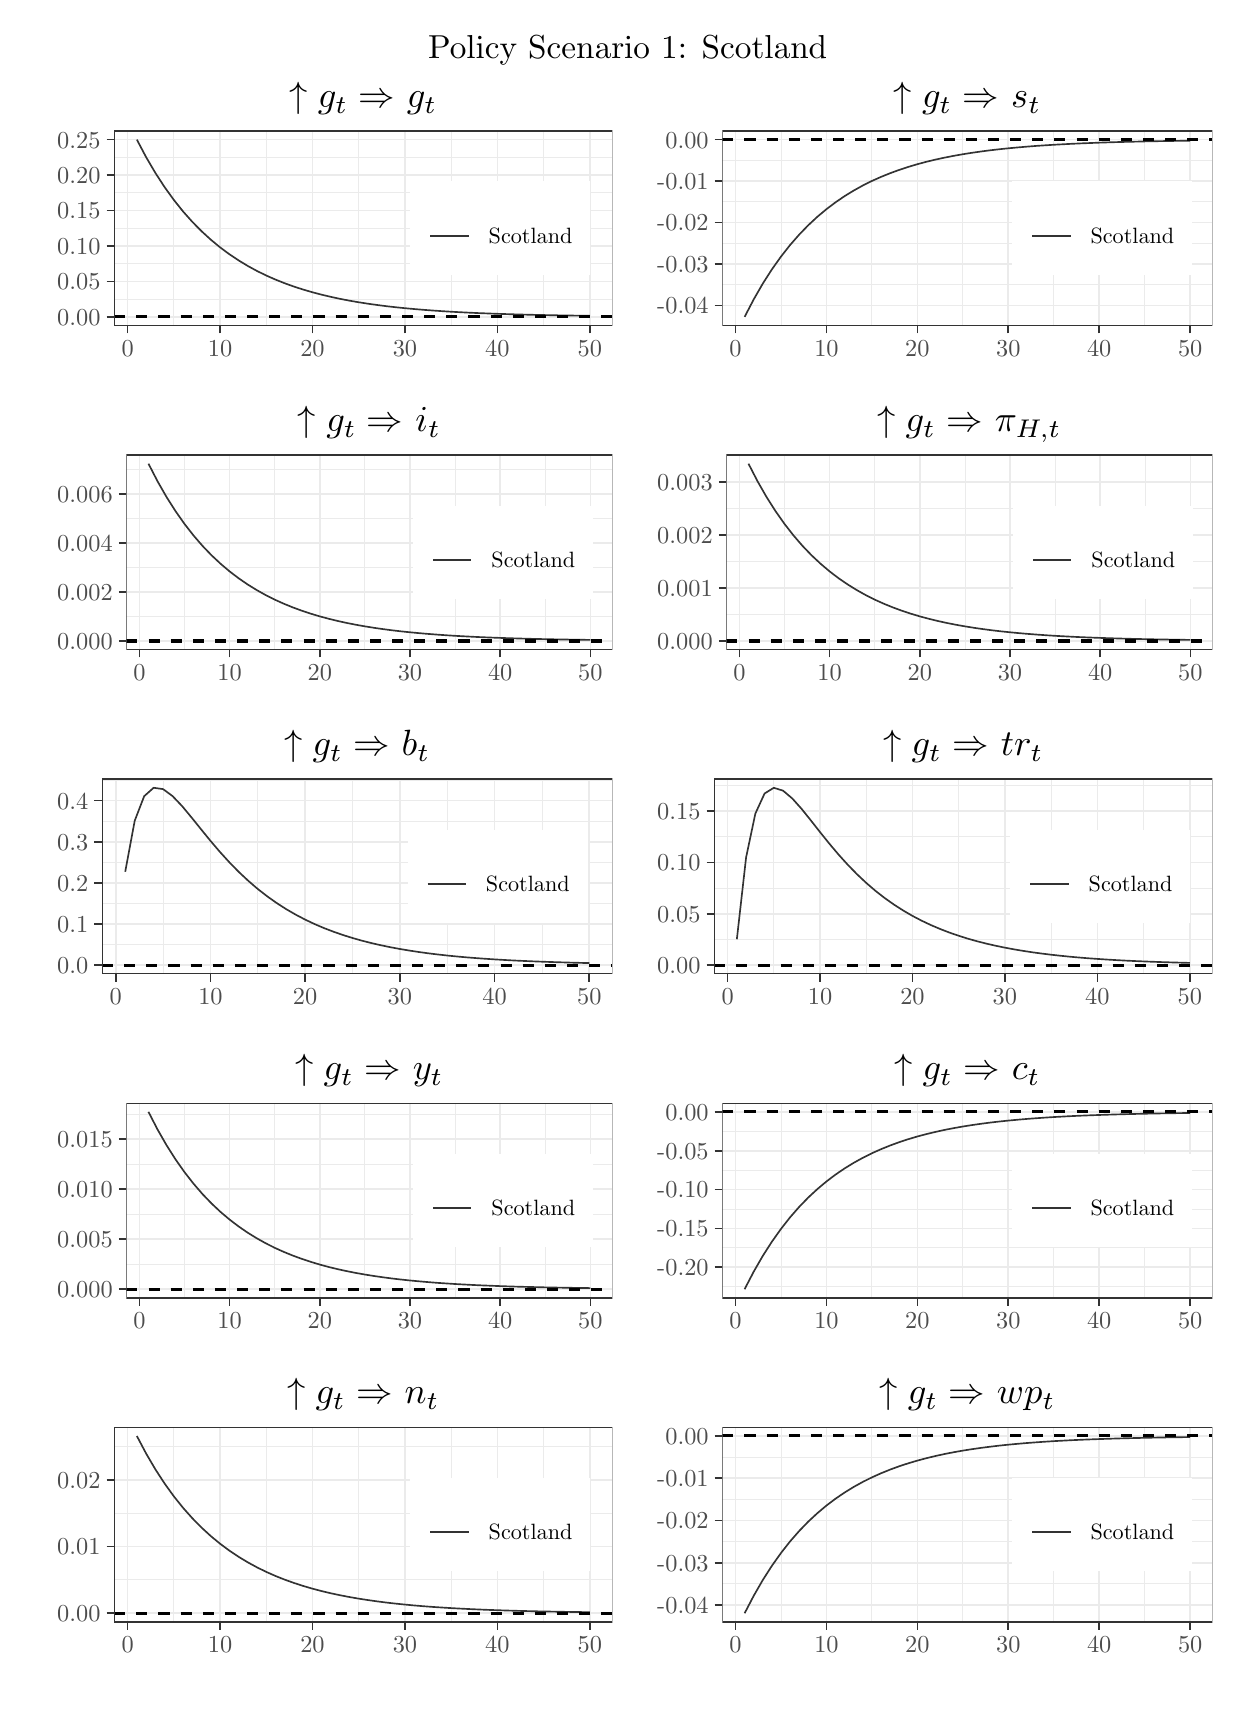
\begin{tikzpicture}[x=1pt,y=1pt]
\definecolor{fillColor}{RGB}{255,255,255}
\path[use as bounding box,fill=fillColor,fill opacity=0.00] (0,0) rectangle (433.62,599.84);
\begin{scope}
\path[clip] (  0.00,468.44) rectangle (216.81,585.55);
\definecolor{drawColor}{RGB}{255,255,255}
\definecolor{fillColor}{RGB}{255,255,255}

\path[draw=drawColor,line width= 0.6pt,line join=round,line cap=round,fill=fillColor] (  0.00,468.44) rectangle (216.81,585.55);
\end{scope}
\begin{scope}
\path[clip] ( 31.27,492.12) rectangle (211.31,562.59);
\definecolor{fillColor}{RGB}{255,255,255}

\path[fill=fillColor] ( 31.27,492.12) rectangle (211.31,562.59);
\definecolor{drawColor}{gray}{0.92}

\path[draw=drawColor,line width= 0.3pt,line join=round] ( 31.27,501.73) --
	(211.31,501.73);

\path[draw=drawColor,line width= 0.3pt,line join=round] ( 31.27,514.54) --
	(211.31,514.54);

\path[draw=drawColor,line width= 0.3pt,line join=round] ( 31.27,527.36) --
	(211.31,527.36);

\path[draw=drawColor,line width= 0.3pt,line join=round] ( 31.27,540.17) --
	(211.31,540.17);

\path[draw=drawColor,line width= 0.3pt,line join=round] ( 31.27,552.98) --
	(211.31,552.98);

\path[draw=drawColor,line width= 0.3pt,line join=round] ( 52.81,492.12) --
	( 52.81,562.59);

\path[draw=drawColor,line width= 0.3pt,line join=round] ( 86.22,492.12) --
	( 86.22,562.59);

\path[draw=drawColor,line width= 0.3pt,line join=round] (119.62,492.12) --
	(119.62,562.59);

\path[draw=drawColor,line width= 0.3pt,line join=round] (153.02,492.12) --
	(153.02,562.59);

\path[draw=drawColor,line width= 0.3pt,line join=round] (186.43,492.12) --
	(186.43,562.59);

\path[draw=drawColor,line width= 0.6pt,line join=round] ( 31.27,495.32) --
	(211.31,495.32);

\path[draw=drawColor,line width= 0.6pt,line join=round] ( 31.27,508.14) --
	(211.31,508.14);

\path[draw=drawColor,line width= 0.6pt,line join=round] ( 31.27,520.95) --
	(211.31,520.95);

\path[draw=drawColor,line width= 0.6pt,line join=round] ( 31.27,533.76) --
	(211.31,533.76);

\path[draw=drawColor,line width= 0.6pt,line join=round] ( 31.27,546.58) --
	(211.31,546.58);

\path[draw=drawColor,line width= 0.6pt,line join=round] ( 31.27,559.39) --
	(211.31,559.39);

\path[draw=drawColor,line width= 0.6pt,line join=round] ( 36.11,492.12) --
	( 36.11,562.59);

\path[draw=drawColor,line width= 0.6pt,line join=round] ( 69.52,492.12) --
	( 69.52,562.59);

\path[draw=drawColor,line width= 0.6pt,line join=round] (102.92,492.12) --
	(102.92,562.59);

\path[draw=drawColor,line width= 0.6pt,line join=round] (136.32,492.12) --
	(136.32,562.59);

\path[draw=drawColor,line width= 0.6pt,line join=round] (169.72,492.12) --
	(169.72,562.59);

\path[draw=drawColor,line width= 0.6pt,line join=round] (203.13,492.12) --
	(203.13,562.59);
\definecolor{drawColor}{gray}{0.20}

\path[draw=drawColor,line width= 0.6pt,line join=round] ( 39.45,559.39) --
	( 42.79,553.06) --
	( 46.13,547.37) --
	( 49.47,542.23) --
	( 52.81,537.60) --
	( 56.15,533.42) --
	( 59.50,529.66) --
	( 62.84,526.27) --
	( 66.18,523.22) --
	( 69.52,520.46) --
	( 72.86,517.98) --
	( 76.20,515.75) --
	( 79.54,513.73) --
	( 82.88,511.91) --
	( 86.22,510.27) --
	( 89.56,508.80) --
	( 92.90,507.47) --
	( 96.24,506.27) --
	( 99.58,505.19) --
	(102.92,504.22) --
	(106.26,503.34) --
	(109.60,502.55) --
	(112.94,501.83) --
	(116.28,501.19) --
	(119.62,500.61) --
	(122.96,500.09) --
	(126.30,499.62) --
	(129.64,499.19) --
	(132.98,498.81) --
	(136.32,498.47) --
	(139.66,498.16) --
	(143.00,497.88) --
	(146.34,497.63) --
	(149.68,497.40) --
	(153.02,497.19) --
	(156.36,497.01) --
	(159.70,496.84) --
	(163.04,496.69) --
	(166.38,496.56) --
	(169.72,496.44) --
	(173.06,496.33) --
	(176.40,496.23) --
	(179.74,496.14) --
	(183.08,496.06) --
	(186.43,495.99) --
	(189.77,495.92) --
	(193.11,495.86) --
	(196.45,495.81) --
	(199.79,495.76) --
	(203.13,495.72);
\definecolor{drawColor}{RGB}{0,0,0}

\path[draw=drawColor,line width= 1.1pt,dash pattern=on 4pt off 4pt ,line join=round] ( 31.27,495.32) -- (211.31,495.32);
\definecolor{drawColor}{gray}{0.20}

\path[draw=drawColor,line width= 0.6pt,line join=round,line cap=round] ( 31.27,492.12) rectangle (211.31,562.59);
\end{scope}
\begin{scope}
\path[clip] (  0.00,  0.00) rectangle (433.62,599.84);
\definecolor{drawColor}{gray}{0.30}

\node[text=drawColor,anchor=base east,inner sep=0pt, outer sep=0pt, scale=  0.88] at ( 26.32,492.29) {0.00};

\node[text=drawColor,anchor=base east,inner sep=0pt, outer sep=0pt, scale=  0.88] at ( 26.32,505.11) {0.05};

\node[text=drawColor,anchor=base east,inner sep=0pt, outer sep=0pt, scale=  0.88] at ( 26.32,517.92) {0.10};

\node[text=drawColor,anchor=base east,inner sep=0pt, outer sep=0pt, scale=  0.88] at ( 26.32,530.73) {0.15};

\node[text=drawColor,anchor=base east,inner sep=0pt, outer sep=0pt, scale=  0.88] at ( 26.32,543.55) {0.20};

\node[text=drawColor,anchor=base east,inner sep=0pt, outer sep=0pt, scale=  0.88] at ( 26.32,556.36) {0.25};
\end{scope}
\begin{scope}
\path[clip] (  0.00,  0.00) rectangle (433.62,599.84);
\definecolor{drawColor}{gray}{0.20}

\path[draw=drawColor,line width= 0.6pt,line join=round] ( 28.52,495.32) --
	( 31.27,495.32);

\path[draw=drawColor,line width= 0.6pt,line join=round] ( 28.52,508.14) --
	( 31.27,508.14);

\path[draw=drawColor,line width= 0.6pt,line join=round] ( 28.52,520.95) --
	( 31.27,520.95);

\path[draw=drawColor,line width= 0.6pt,line join=round] ( 28.52,533.76) --
	( 31.27,533.76);

\path[draw=drawColor,line width= 0.6pt,line join=round] ( 28.52,546.58) --
	( 31.27,546.58);

\path[draw=drawColor,line width= 0.6pt,line join=round] ( 28.52,559.39) --
	( 31.27,559.39);
\end{scope}
\begin{scope}
\path[clip] (  0.00,  0.00) rectangle (433.62,599.84);
\definecolor{drawColor}{gray}{0.20}

\path[draw=drawColor,line width= 0.6pt,line join=round] ( 36.11,489.37) --
	( 36.11,492.12);

\path[draw=drawColor,line width= 0.6pt,line join=round] ( 69.52,489.37) --
	( 69.52,492.12);

\path[draw=drawColor,line width= 0.6pt,line join=round] (102.92,489.37) --
	(102.92,492.12);

\path[draw=drawColor,line width= 0.6pt,line join=round] (136.32,489.37) --
	(136.32,492.12);

\path[draw=drawColor,line width= 0.6pt,line join=round] (169.72,489.37) --
	(169.72,492.12);

\path[draw=drawColor,line width= 0.6pt,line join=round] (203.13,489.37) --
	(203.13,492.12);
\end{scope}
\begin{scope}
\path[clip] (  0.00,  0.00) rectangle (433.62,599.84);
\definecolor{drawColor}{gray}{0.30}

\node[text=drawColor,anchor=base,inner sep=0pt, outer sep=0pt, scale=  0.88] at ( 36.11,481.11) {0};

\node[text=drawColor,anchor=base,inner sep=0pt, outer sep=0pt, scale=  0.88] at ( 69.52,481.11) {10};

\node[text=drawColor,anchor=base,inner sep=0pt, outer sep=0pt, scale=  0.88] at (102.92,481.11) {20};

\node[text=drawColor,anchor=base,inner sep=0pt, outer sep=0pt, scale=  0.88] at (136.32,481.11) {30};

\node[text=drawColor,anchor=base,inner sep=0pt, outer sep=0pt, scale=  0.88] at (169.72,481.11) {40};

\node[text=drawColor,anchor=base,inner sep=0pt, outer sep=0pt, scale=  0.88] at (203.13,481.11) {50};
\end{scope}
\begin{scope}
\path[clip] (  0.00,  0.00) rectangle (433.62,599.84);
\definecolor{fillColor}{RGB}{255,255,255}

\path[fill=fillColor] (138.26,510.43) rectangle (203.35,544.28);
\end{scope}
\begin{scope}
\path[clip] (  0.00,  0.00) rectangle (433.62,599.84);
\definecolor{fillColor}{RGB}{255,255,255}

\path[fill=fillColor] (143.76,515.93) rectangle (161.10,533.28);
\end{scope}
\begin{scope}
\path[clip] (  0.00,  0.00) rectangle (433.62,599.84);
\definecolor{drawColor}{gray}{0.20}

\path[draw=drawColor,line width= 0.6pt,line join=round] (145.49,524.61) -- (159.37,524.61);
\end{scope}
\begin{scope}
\path[clip] (  0.00,  0.00) rectangle (433.62,599.84);
\definecolor{drawColor}{RGB}{0,0,0}

\node[text=drawColor,anchor=base west,inner sep=0pt, outer sep=0pt, scale=  0.80] at (166.60,521.85) {Scotland};
\end{scope}
\begin{scope}
\path[clip] (  0.00,  0.00) rectangle (433.62,599.84);
\definecolor{drawColor}{RGB}{0,0,0}

\node[text=drawColor,anchor=base,inner sep=0pt, outer sep=0pt, scale=  1.32] at (121.29,570.96) {$\uparrow  g_t \Rightarrow $ ${g_t}$};
\end{scope}
\begin{scope}
\path[clip] (216.81,468.44) rectangle (433.62,585.55);
\definecolor{drawColor}{RGB}{255,255,255}
\definecolor{fillColor}{RGB}{255,255,255}

\path[draw=drawColor,line width= 0.6pt,line join=round,line cap=round,fill=fillColor] (216.81,468.44) rectangle (433.62,585.55);
\end{scope}
\begin{scope}
\path[clip] (251.01,492.12) rectangle (428.12,562.59);
\definecolor{fillColor}{RGB}{255,255,255}

\path[fill=fillColor] (251.01,492.12) rectangle (428.12,562.59);
\definecolor{drawColor}{gray}{0.92}

\path[draw=drawColor,line width= 0.3pt,line join=round] (251.01,506.95) --
	(428.12,506.95);

\path[draw=drawColor,line width= 0.3pt,line join=round] (251.01,521.93) --
	(428.12,521.93);

\path[draw=drawColor,line width= 0.3pt,line join=round] (251.01,536.91) --
	(428.12,536.91);

\path[draw=drawColor,line width= 0.3pt,line join=round] (251.01,551.90) --
	(428.12,551.90);

\path[draw=drawColor,line width= 0.3pt,line join=round] (272.21,492.12) --
	(272.21,562.59);

\path[draw=drawColor,line width= 0.3pt,line join=round] (305.06,492.12) --
	(305.06,562.59);

\path[draw=drawColor,line width= 0.3pt,line join=round] (337.92,492.12) --
	(337.92,562.59);

\path[draw=drawColor,line width= 0.3pt,line join=round] (370.78,492.12) --
	(370.78,562.59);

\path[draw=drawColor,line width= 0.3pt,line join=round] (403.64,492.12) --
	(403.64,562.59);

\path[draw=drawColor,line width= 0.6pt,line join=round] (251.01,499.45) --
	(428.12,499.45);

\path[draw=drawColor,line width= 0.6pt,line join=round] (251.01,514.44) --
	(428.12,514.44);

\path[draw=drawColor,line width= 0.6pt,line join=round] (251.01,529.42) --
	(428.12,529.42);

\path[draw=drawColor,line width= 0.6pt,line join=round] (251.01,544.41) --
	(428.12,544.41);

\path[draw=drawColor,line width= 0.6pt,line join=round] (251.01,559.39) --
	(428.12,559.39);

\path[draw=drawColor,line width= 0.6pt,line join=round] (255.78,492.12) --
	(255.78,562.59);

\path[draw=drawColor,line width= 0.6pt,line join=round] (288.64,492.12) --
	(288.64,562.59);

\path[draw=drawColor,line width= 0.6pt,line join=round] (321.49,492.12) --
	(321.49,562.59);

\path[draw=drawColor,line width= 0.6pt,line join=round] (354.35,492.12) --
	(354.35,562.59);

\path[draw=drawColor,line width= 0.6pt,line join=round] (387.21,492.12) --
	(387.21,562.59);

\path[draw=drawColor,line width= 0.6pt,line join=round] (420.07,492.12) --
	(420.07,562.59);
\definecolor{drawColor}{gray}{0.20}

\path[draw=drawColor,line width= 0.6pt,line join=round] (259.06,495.32) --
	(262.35,501.65) --
	(265.63,507.35) --
	(268.92,512.49) --
	(272.21,517.12) --
	(275.49,521.29) --
	(278.78,525.05) --
	(282.06,528.44) --
	(285.35,531.50) --
	(288.64,534.25) --
	(291.92,536.73) --
	(295.21,538.97) --
	(298.49,540.98) --
	(301.78,542.80) --
	(305.06,544.44) --
	(308.35,545.91) --
	(311.64,547.24) --
	(314.92,548.44) --
	(318.21,549.52) --
	(321.49,550.50) --
	(324.78,551.38) --
	(328.07,552.17) --
	(331.35,552.88) --
	(334.64,553.52) --
	(337.92,554.10) --
	(341.21,554.62) --
	(344.49,555.09) --
	(347.78,555.52) --
	(351.07,555.90) --
	(354.35,556.24) --
	(357.64,556.55) --
	(360.92,556.83) --
	(364.21,557.09) --
	(367.50,557.31) --
	(370.78,557.52) --
	(374.07,557.70) --
	(377.35,557.87) --
	(380.64,558.02) --
	(383.93,558.15) --
	(387.21,558.28) --
	(390.50,558.39) --
	(393.78,558.49) --
	(397.07,558.57) --
	(400.35,558.65) --
	(403.64,558.73) --
	(406.93,558.79) --
	(410.21,558.85) --
	(413.50,558.90) --
	(416.78,558.95) --
	(420.07,559.00);
\definecolor{drawColor}{RGB}{0,0,0}

\path[draw=drawColor,line width= 1.1pt,dash pattern=on 4pt off 4pt ,line join=round] (251.01,559.39) -- (428.12,559.39);
\definecolor{drawColor}{gray}{0.20}

\path[draw=drawColor,line width= 0.6pt,line join=round,line cap=round] (251.01,492.12) rectangle (428.12,562.59);
\end{scope}
\begin{scope}
\path[clip] (  0.00,  0.00) rectangle (433.62,599.84);
\definecolor{drawColor}{gray}{0.30}

\node[text=drawColor,anchor=base east,inner sep=0pt, outer sep=0pt, scale=  0.88] at (246.06,496.42) {-0.04};

\node[text=drawColor,anchor=base east,inner sep=0pt, outer sep=0pt, scale=  0.88] at (246.06,511.41) {-0.03};

\node[text=drawColor,anchor=base east,inner sep=0pt, outer sep=0pt, scale=  0.88] at (246.06,526.39) {-0.02};

\node[text=drawColor,anchor=base east,inner sep=0pt, outer sep=0pt, scale=  0.88] at (246.06,541.37) {-0.01};

\node[text=drawColor,anchor=base east,inner sep=0pt, outer sep=0pt, scale=  0.88] at (246.06,556.36) {0.00};
\end{scope}
\begin{scope}
\path[clip] (  0.00,  0.00) rectangle (433.62,599.84);
\definecolor{drawColor}{gray}{0.20}

\path[draw=drawColor,line width= 0.6pt,line join=round] (248.26,499.45) --
	(251.01,499.45);

\path[draw=drawColor,line width= 0.6pt,line join=round] (248.26,514.44) --
	(251.01,514.44);

\path[draw=drawColor,line width= 0.6pt,line join=round] (248.26,529.42) --
	(251.01,529.42);

\path[draw=drawColor,line width= 0.6pt,line join=round] (248.26,544.41) --
	(251.01,544.41);

\path[draw=drawColor,line width= 0.6pt,line join=round] (248.26,559.39) --
	(251.01,559.39);
\end{scope}
\begin{scope}
\path[clip] (  0.00,  0.00) rectangle (433.62,599.84);
\definecolor{drawColor}{gray}{0.20}

\path[draw=drawColor,line width= 0.6pt,line join=round] (255.78,489.37) --
	(255.78,492.12);

\path[draw=drawColor,line width= 0.6pt,line join=round] (288.64,489.37) --
	(288.64,492.12);

\path[draw=drawColor,line width= 0.6pt,line join=round] (321.49,489.37) --
	(321.49,492.12);

\path[draw=drawColor,line width= 0.6pt,line join=round] (354.35,489.37) --
	(354.35,492.12);

\path[draw=drawColor,line width= 0.6pt,line join=round] (387.21,489.37) --
	(387.21,492.12);

\path[draw=drawColor,line width= 0.6pt,line join=round] (420.07,489.37) --
	(420.07,492.12);
\end{scope}
\begin{scope}
\path[clip] (  0.00,  0.00) rectangle (433.62,599.84);
\definecolor{drawColor}{gray}{0.30}

\node[text=drawColor,anchor=base,inner sep=0pt, outer sep=0pt, scale=  0.88] at (255.78,481.11) {0};

\node[text=drawColor,anchor=base,inner sep=0pt, outer sep=0pt, scale=  0.88] at (288.64,481.11) {10};

\node[text=drawColor,anchor=base,inner sep=0pt, outer sep=0pt, scale=  0.88] at (321.49,481.11) {20};

\node[text=drawColor,anchor=base,inner sep=0pt, outer sep=0pt, scale=  0.88] at (354.35,481.11) {30};

\node[text=drawColor,anchor=base,inner sep=0pt, outer sep=0pt, scale=  0.88] at (387.21,481.11) {40};

\node[text=drawColor,anchor=base,inner sep=0pt, outer sep=0pt, scale=  0.88] at (420.07,481.11) {50};
\end{scope}
\begin{scope}
\path[clip] (  0.00,  0.00) rectangle (433.62,599.84);
\definecolor{fillColor}{RGB}{255,255,255}

\path[fill=fillColor] (355.73,510.43) rectangle (420.82,544.28);
\end{scope}
\begin{scope}
\path[clip] (  0.00,  0.00) rectangle (433.62,599.84);
\definecolor{fillColor}{RGB}{255,255,255}

\path[fill=fillColor] (361.23,515.93) rectangle (378.57,533.28);
\end{scope}
\begin{scope}
\path[clip] (  0.00,  0.00) rectangle (433.62,599.84);
\definecolor{drawColor}{gray}{0.20}

\path[draw=drawColor,line width= 0.6pt,line join=round] (362.96,524.61) -- (376.84,524.61);
\end{scope}
\begin{scope}
\path[clip] (  0.00,  0.00) rectangle (433.62,599.84);
\definecolor{drawColor}{RGB}{0,0,0}

\node[text=drawColor,anchor=base west,inner sep=0pt, outer sep=0pt, scale=  0.80] at (384.07,521.85) {Scotland};
\end{scope}
\begin{scope}
\path[clip] (  0.00,  0.00) rectangle (433.62,599.84);
\definecolor{drawColor}{RGB}{0,0,0}

\node[text=drawColor,anchor=base,inner sep=0pt, outer sep=0pt, scale=  1.32] at (339.57,570.96) {$\uparrow  g_t \Rightarrow $ ${s_t}$};
\end{scope}
\begin{scope}
\path[clip] (  0.00,351.33) rectangle (216.81,468.44);
\definecolor{drawColor}{RGB}{255,255,255}
\definecolor{fillColor}{RGB}{255,255,255}

\path[draw=drawColor,line width= 0.6pt,line join=round,line cap=round,fill=fillColor] (  0.00,351.33) rectangle (216.81,468.44);
\end{scope}
\begin{scope}
\path[clip] ( 35.67,375.01) rectangle (211.31,445.48);
\definecolor{fillColor}{RGB}{255,255,255}

\path[fill=fillColor] ( 35.67,375.01) rectangle (211.31,445.48);
\definecolor{drawColor}{gray}{0.92}

\path[draw=drawColor,line width= 0.3pt,line join=round] ( 35.67,387.06) --
	(211.31,387.06);

\path[draw=drawColor,line width= 0.3pt,line join=round] ( 35.67,404.75) --
	(211.31,404.75);

\path[draw=drawColor,line width= 0.3pt,line join=round] ( 35.67,422.45) --
	(211.31,422.45);

\path[draw=drawColor,line width= 0.3pt,line join=round] ( 35.67,440.14) --
	(211.31,440.14);

\path[draw=drawColor,line width= 0.3pt,line join=round] ( 56.69,375.01) --
	( 56.69,445.48);

\path[draw=drawColor,line width= 0.3pt,line join=round] ( 89.27,375.01) --
	( 89.27,445.48);

\path[draw=drawColor,line width= 0.3pt,line join=round] (121.86,375.01) --
	(121.86,445.48);

\path[draw=drawColor,line width= 0.3pt,line join=round] (154.45,375.01) --
	(154.45,445.48);

\path[draw=drawColor,line width= 0.3pt,line join=round] (187.03,375.01) --
	(187.03,445.48);

\path[draw=drawColor,line width= 0.6pt,line join=round] ( 35.67,378.21) --
	(211.31,378.21);

\path[draw=drawColor,line width= 0.6pt,line join=round] ( 35.67,395.91) --
	(211.31,395.91);

\path[draw=drawColor,line width= 0.6pt,line join=round] ( 35.67,413.60) --
	(211.31,413.60);

\path[draw=drawColor,line width= 0.6pt,line join=round] ( 35.67,431.29) --
	(211.31,431.29);

\path[draw=drawColor,line width= 0.6pt,line join=round] ( 40.39,375.01) --
	( 40.39,445.48);

\path[draw=drawColor,line width= 0.6pt,line join=round] ( 72.98,375.01) --
	( 72.98,445.48);

\path[draw=drawColor,line width= 0.6pt,line join=round] (105.57,375.01) --
	(105.57,445.48);

\path[draw=drawColor,line width= 0.6pt,line join=round] (138.15,375.01) --
	(138.15,445.48);

\path[draw=drawColor,line width= 0.6pt,line join=round] (170.74,375.01) --
	(170.74,445.48);

\path[draw=drawColor,line width= 0.6pt,line join=round] (203.33,375.01) --
	(203.33,445.48);
\definecolor{drawColor}{gray}{0.20}

\path[draw=drawColor,line width= 0.6pt,line join=round] ( 43.65,442.28) --
	( 46.91,435.95) --
	( 50.17,430.25) --
	( 53.43,425.12) --
	( 56.69,420.49) --
	( 59.95,416.31) --
	( 63.20,412.55) --
	( 66.46,409.16) --
	( 69.72,406.11) --
	( 72.98,403.35) --
	( 76.24,400.87) --
	( 79.50,398.63) --
	( 82.76,396.62) --
	( 86.01,394.80) --
	( 89.27,393.16) --
	( 92.53,391.69) --
	( 95.79,390.36) --
	( 99.05,389.16) --
	(102.31,388.08) --
	(105.57,387.10) --
	(108.83,386.23) --
	(112.08,385.44) --
	(115.34,384.72) --
	(118.60,384.08) --
	(121.86,383.50) --
	(125.12,382.98) --
	(128.38,382.51) --
	(131.64,382.08) --
	(134.89,381.70) --
	(138.15,381.36) --
	(141.41,381.05) --
	(144.67,380.77) --
	(147.93,380.52) --
	(151.19,380.29) --
	(154.45,380.08) --
	(157.71,379.90) --
	(160.96,379.73) --
	(164.22,379.58) --
	(167.48,379.45) --
	(170.74,379.33) --
	(174.00,379.22) --
	(177.26,379.12) --
	(180.52,379.03) --
	(183.77,378.95) --
	(187.03,378.87) --
	(190.29,378.81) --
	(193.55,378.75) --
	(196.81,378.70) --
	(200.07,378.65) --
	(203.33,378.61);
\definecolor{drawColor}{RGB}{0,0,0}

\path[draw=drawColor,line width= 1.1pt,dash pattern=on 4pt off 4pt ,line join=round] ( 35.67,378.21) -- (211.31,378.21);
\definecolor{drawColor}{gray}{0.20}

\path[draw=drawColor,line width= 0.6pt,line join=round,line cap=round] ( 35.67,375.01) rectangle (211.31,445.48);
\end{scope}
\begin{scope}
\path[clip] (  0.00,  0.00) rectangle (433.62,599.84);
\definecolor{drawColor}{gray}{0.30}

\node[text=drawColor,anchor=base east,inner sep=0pt, outer sep=0pt, scale=  0.88] at ( 30.72,375.18) {0.000};

\node[text=drawColor,anchor=base east,inner sep=0pt, outer sep=0pt, scale=  0.88] at ( 30.72,392.88) {0.002};

\node[text=drawColor,anchor=base east,inner sep=0pt, outer sep=0pt, scale=  0.88] at ( 30.72,410.57) {0.004};

\node[text=drawColor,anchor=base east,inner sep=0pt, outer sep=0pt, scale=  0.88] at ( 30.72,428.26) {0.006};
\end{scope}
\begin{scope}
\path[clip] (  0.00,  0.00) rectangle (433.62,599.84);
\definecolor{drawColor}{gray}{0.20}

\path[draw=drawColor,line width= 0.6pt,line join=round] ( 32.92,378.21) --
	( 35.67,378.21);

\path[draw=drawColor,line width= 0.6pt,line join=round] ( 32.92,395.91) --
	( 35.67,395.91);

\path[draw=drawColor,line width= 0.6pt,line join=round] ( 32.92,413.60) --
	( 35.67,413.60);

\path[draw=drawColor,line width= 0.6pt,line join=round] ( 32.92,431.29) --
	( 35.67,431.29);
\end{scope}
\begin{scope}
\path[clip] (  0.00,  0.00) rectangle (433.62,599.84);
\definecolor{drawColor}{gray}{0.20}

\path[draw=drawColor,line width= 0.6pt,line join=round] ( 40.39,372.26) --
	( 40.39,375.01);

\path[draw=drawColor,line width= 0.6pt,line join=round] ( 72.98,372.26) --
	( 72.98,375.01);

\path[draw=drawColor,line width= 0.6pt,line join=round] (105.57,372.26) --
	(105.57,375.01);

\path[draw=drawColor,line width= 0.6pt,line join=round] (138.15,372.26) --
	(138.15,375.01);

\path[draw=drawColor,line width= 0.6pt,line join=round] (170.74,372.26) --
	(170.74,375.01);

\path[draw=drawColor,line width= 0.6pt,line join=round] (203.33,372.26) --
	(203.33,375.01);
\end{scope}
\begin{scope}
\path[clip] (  0.00,  0.00) rectangle (433.62,599.84);
\definecolor{drawColor}{gray}{0.30}

\node[text=drawColor,anchor=base,inner sep=0pt, outer sep=0pt, scale=  0.88] at ( 40.39,364.00) {0};

\node[text=drawColor,anchor=base,inner sep=0pt, outer sep=0pt, scale=  0.88] at ( 72.98,364.00) {10};

\node[text=drawColor,anchor=base,inner sep=0pt, outer sep=0pt, scale=  0.88] at (105.57,364.00) {20};

\node[text=drawColor,anchor=base,inner sep=0pt, outer sep=0pt, scale=  0.88] at (138.15,364.00) {30};

\node[text=drawColor,anchor=base,inner sep=0pt, outer sep=0pt, scale=  0.88] at (170.74,364.00) {40};

\node[text=drawColor,anchor=base,inner sep=0pt, outer sep=0pt, scale=  0.88] at (203.33,364.00) {50};
\end{scope}
\begin{scope}
\path[clip] (  0.00,  0.00) rectangle (433.62,599.84);
\definecolor{fillColor}{RGB}{255,255,255}

\path[fill=fillColor] (139.25,393.32) rectangle (204.34,427.17);
\end{scope}
\begin{scope}
\path[clip] (  0.00,  0.00) rectangle (433.62,599.84);
\definecolor{fillColor}{RGB}{255,255,255}

\path[fill=fillColor] (144.75,398.82) rectangle (162.09,416.17);
\end{scope}
\begin{scope}
\path[clip] (  0.00,  0.00) rectangle (433.62,599.84);
\definecolor{drawColor}{gray}{0.20}

\path[draw=drawColor,line width= 0.6pt,line join=round] (146.48,407.50) -- (160.36,407.50);
\end{scope}
\begin{scope}
\path[clip] (  0.00,  0.00) rectangle (433.62,599.84);
\definecolor{drawColor}{RGB}{0,0,0}

\node[text=drawColor,anchor=base west,inner sep=0pt, outer sep=0pt, scale=  0.80] at (167.59,404.74) {Scotland};
\end{scope}
\begin{scope}
\path[clip] (  0.00,  0.00) rectangle (433.62,599.84);
\definecolor{drawColor}{RGB}{0,0,0}

\node[text=drawColor,anchor=base,inner sep=0pt, outer sep=0pt, scale=  1.32] at (123.49,453.85) {$\uparrow  g_t \Rightarrow $ ${i_t}$};
\end{scope}
\begin{scope}
\path[clip] (216.81,351.33) rectangle (433.62,468.44);
\definecolor{drawColor}{RGB}{255,255,255}
\definecolor{fillColor}{RGB}{255,255,255}

\path[draw=drawColor,line width= 0.6pt,line join=round,line cap=round,fill=fillColor] (216.81,351.33) rectangle (433.62,468.44);
\end{scope}
\begin{scope}
\path[clip] (252.48,375.01) rectangle (428.12,445.48);
\definecolor{fillColor}{RGB}{255,255,255}

\path[fill=fillColor] (252.48,375.01) rectangle (428.12,445.48);
\definecolor{drawColor}{gray}{0.92}

\path[draw=drawColor,line width= 0.3pt,line join=round] (252.48,387.77) --
	(428.12,387.77);

\path[draw=drawColor,line width= 0.3pt,line join=round] (252.48,406.88) --
	(428.12,406.88);

\path[draw=drawColor,line width= 0.3pt,line join=round] (252.48,426.00) --
	(428.12,426.00);

\path[draw=drawColor,line width= 0.3pt,line join=round] (252.48,445.11) --
	(428.12,445.11);

\path[draw=drawColor,line width= 0.3pt,line join=round] (273.50,375.01) --
	(273.50,445.48);

\path[draw=drawColor,line width= 0.3pt,line join=round] (306.08,375.01) --
	(306.08,445.48);

\path[draw=drawColor,line width= 0.3pt,line join=round] (338.67,375.01) --
	(338.67,445.48);

\path[draw=drawColor,line width= 0.3pt,line join=round] (371.26,375.01) --
	(371.26,445.48);

\path[draw=drawColor,line width= 0.3pt,line join=round] (403.84,375.01) --
	(403.84,445.48);

\path[draw=drawColor,line width= 0.6pt,line join=round] (252.48,378.21) --
	(428.12,378.21);

\path[draw=drawColor,line width= 0.6pt,line join=round] (252.48,397.33) --
	(428.12,397.33);

\path[draw=drawColor,line width= 0.6pt,line join=round] (252.48,416.44) --
	(428.12,416.44);

\path[draw=drawColor,line width= 0.6pt,line join=round] (252.48,435.55) --
	(428.12,435.55);

\path[draw=drawColor,line width= 0.6pt,line join=round] (257.20,375.01) --
	(257.20,445.48);

\path[draw=drawColor,line width= 0.6pt,line join=round] (289.79,375.01) --
	(289.79,445.48);

\path[draw=drawColor,line width= 0.6pt,line join=round] (322.38,375.01) --
	(322.38,445.48);

\path[draw=drawColor,line width= 0.6pt,line join=round] (354.96,375.01) --
	(354.96,445.48);

\path[draw=drawColor,line width= 0.6pt,line join=round] (387.55,375.01) --
	(387.55,445.48);

\path[draw=drawColor,line width= 0.6pt,line join=round] (420.14,375.01) --
	(420.14,445.48);
\definecolor{drawColor}{gray}{0.20}

\path[draw=drawColor,line width= 0.6pt,line join=round] (260.46,442.28) --
	(263.72,435.95) --
	(266.98,430.25) --
	(270.24,425.12) --
	(273.50,420.49) --
	(276.76,416.31) --
	(280.01,412.55) --
	(283.27,409.16) --
	(286.53,406.11) --
	(289.79,403.35) --
	(293.05,400.87) --
	(296.31,398.64) --
	(299.57,396.62) --
	(302.82,394.80) --
	(306.08,393.16) --
	(309.34,391.69) --
	(312.60,390.36) --
	(315.86,389.16) --
	(319.12,388.08) --
	(322.38,387.10) --
	(325.64,386.23) --
	(328.89,385.44) --
	(332.15,384.72) --
	(335.41,384.08) --
	(338.67,383.50) --
	(341.93,382.98) --
	(345.19,382.51) --
	(348.45,382.08) --
	(351.70,381.70) --
	(354.96,381.36) --
	(358.22,381.05) --
	(361.48,380.77) --
	(364.74,380.52) --
	(368.00,380.29) --
	(371.26,380.08) --
	(374.52,379.90) --
	(377.77,379.73) --
	(381.03,379.58) --
	(384.29,379.45) --
	(387.55,379.33) --
	(390.81,379.22) --
	(394.07,379.12) --
	(397.33,379.03) --
	(400.58,378.95) --
	(403.84,378.87) --
	(407.10,378.81) --
	(410.36,378.75) --
	(413.62,378.70) --
	(416.88,378.65) --
	(420.14,378.61);
\definecolor{drawColor}{RGB}{0,0,0}

\path[draw=drawColor,line width= 1.1pt,dash pattern=on 4pt off 4pt ,line join=round] (252.48,378.21) -- (428.12,378.21);
\definecolor{drawColor}{gray}{0.20}

\path[draw=drawColor,line width= 0.6pt,line join=round,line cap=round] (252.48,375.01) rectangle (428.12,445.48);
\end{scope}
\begin{scope}
\path[clip] (  0.00,  0.00) rectangle (433.62,599.84);
\definecolor{drawColor}{gray}{0.30}

\node[text=drawColor,anchor=base east,inner sep=0pt, outer sep=0pt, scale=  0.88] at (247.53,375.18) {0.000};

\node[text=drawColor,anchor=base east,inner sep=0pt, outer sep=0pt, scale=  0.88] at (247.53,394.30) {0.001};

\node[text=drawColor,anchor=base east,inner sep=0pt, outer sep=0pt, scale=  0.88] at (247.53,413.41) {0.002};

\node[text=drawColor,anchor=base east,inner sep=0pt, outer sep=0pt, scale=  0.88] at (247.53,432.52) {0.003};
\end{scope}
\begin{scope}
\path[clip] (  0.00,  0.00) rectangle (433.62,599.84);
\definecolor{drawColor}{gray}{0.20}

\path[draw=drawColor,line width= 0.6pt,line join=round] (249.73,378.21) --
	(252.48,378.21);

\path[draw=drawColor,line width= 0.6pt,line join=round] (249.73,397.33) --
	(252.48,397.33);

\path[draw=drawColor,line width= 0.6pt,line join=round] (249.73,416.44) --
	(252.48,416.44);

\path[draw=drawColor,line width= 0.6pt,line join=round] (249.73,435.55) --
	(252.48,435.55);
\end{scope}
\begin{scope}
\path[clip] (  0.00,  0.00) rectangle (433.62,599.84);
\definecolor{drawColor}{gray}{0.20}

\path[draw=drawColor,line width= 0.6pt,line join=round] (257.20,372.26) --
	(257.20,375.01);

\path[draw=drawColor,line width= 0.6pt,line join=round] (289.79,372.26) --
	(289.79,375.01);

\path[draw=drawColor,line width= 0.6pt,line join=round] (322.38,372.26) --
	(322.38,375.01);

\path[draw=drawColor,line width= 0.6pt,line join=round] (354.96,372.26) --
	(354.96,375.01);

\path[draw=drawColor,line width= 0.6pt,line join=round] (387.55,372.26) --
	(387.55,375.01);

\path[draw=drawColor,line width= 0.6pt,line join=round] (420.14,372.26) --
	(420.14,375.01);
\end{scope}
\begin{scope}
\path[clip] (  0.00,  0.00) rectangle (433.62,599.84);
\definecolor{drawColor}{gray}{0.30}

\node[text=drawColor,anchor=base,inner sep=0pt, outer sep=0pt, scale=  0.88] at (257.20,364.00) {0};

\node[text=drawColor,anchor=base,inner sep=0pt, outer sep=0pt, scale=  0.88] at (289.79,364.00) {10};

\node[text=drawColor,anchor=base,inner sep=0pt, outer sep=0pt, scale=  0.88] at (322.38,364.00) {20};

\node[text=drawColor,anchor=base,inner sep=0pt, outer sep=0pt, scale=  0.88] at (354.96,364.00) {30};

\node[text=drawColor,anchor=base,inner sep=0pt, outer sep=0pt, scale=  0.88] at (387.55,364.00) {40};

\node[text=drawColor,anchor=base,inner sep=0pt, outer sep=0pt, scale=  0.88] at (420.14,364.00) {50};
\end{scope}
\begin{scope}
\path[clip] (  0.00,  0.00) rectangle (433.62,599.84);
\definecolor{fillColor}{RGB}{255,255,255}

\path[fill=fillColor] (356.06,393.32) rectangle (421.15,427.17);
\end{scope}
\begin{scope}
\path[clip] (  0.00,  0.00) rectangle (433.62,599.84);
\definecolor{fillColor}{RGB}{255,255,255}

\path[fill=fillColor] (361.56,398.82) rectangle (378.90,416.17);
\end{scope}
\begin{scope}
\path[clip] (  0.00,  0.00) rectangle (433.62,599.84);
\definecolor{drawColor}{gray}{0.20}

\path[draw=drawColor,line width= 0.6pt,line join=round] (363.29,407.50) -- (377.17,407.50);
\end{scope}
\begin{scope}
\path[clip] (  0.00,  0.00) rectangle (433.62,599.84);
\definecolor{drawColor}{RGB}{0,0,0}

\node[text=drawColor,anchor=base west,inner sep=0pt, outer sep=0pt, scale=  0.80] at (384.40,404.74) {Scotland};
\end{scope}
\begin{scope}
\path[clip] (  0.00,  0.00) rectangle (433.62,599.84);
\definecolor{drawColor}{RGB}{0,0,0}

\node[text=drawColor,anchor=base,inner sep=0pt, outer sep=0pt, scale=  1.32] at (340.30,453.85) {$\uparrow  g_t \Rightarrow $ ${\pi_{H,t}}$};
\end{scope}
\begin{scope}
\path[clip] (  0.00,234.22) rectangle (216.81,351.33);
\definecolor{drawColor}{RGB}{255,255,255}
\definecolor{fillColor}{RGB}{255,255,255}

\path[draw=drawColor,line width= 0.6pt,line join=round,line cap=round,fill=fillColor] (  0.00,234.22) rectangle (216.81,351.33);
\end{scope}
\begin{scope}
\path[clip] ( 26.87,257.90) rectangle (211.31,328.37);
\definecolor{fillColor}{RGB}{255,255,255}

\path[fill=fillColor] ( 26.87,257.90) rectangle (211.31,328.37);
\definecolor{drawColor}{gray}{0.92}

\path[draw=drawColor,line width= 0.3pt,line join=round] ( 26.87,268.53) --
	(211.31,268.53);

\path[draw=drawColor,line width= 0.3pt,line join=round] ( 26.87,283.38) --
	(211.31,283.38);

\path[draw=drawColor,line width= 0.3pt,line join=round] ( 26.87,298.24) --
	(211.31,298.24);

\path[draw=drawColor,line width= 0.3pt,line join=round] ( 26.87,313.09) --
	(211.31,313.09);

\path[draw=drawColor,line width= 0.3pt,line join=round] ( 26.87,327.94) --
	(211.31,327.94);

\path[draw=drawColor,line width= 0.3pt,line join=round] ( 48.94,257.90) --
	( 48.94,328.37);

\path[draw=drawColor,line width= 0.3pt,line join=round] ( 83.16,257.90) --
	( 83.16,328.37);

\path[draw=drawColor,line width= 0.3pt,line join=round] (117.38,257.90) --
	(117.38,328.37);

\path[draw=drawColor,line width= 0.3pt,line join=round] (151.60,257.90) --
	(151.60,328.37);

\path[draw=drawColor,line width= 0.3pt,line join=round] (185.82,257.90) --
	(185.82,328.37);

\path[draw=drawColor,line width= 0.6pt,line join=round] ( 26.87,261.10) --
	(211.31,261.10);

\path[draw=drawColor,line width= 0.6pt,line join=round] ( 26.87,275.96) --
	(211.31,275.96);

\path[draw=drawColor,line width= 0.6pt,line join=round] ( 26.87,290.81) --
	(211.31,290.81);

\path[draw=drawColor,line width= 0.6pt,line join=round] ( 26.87,305.66) --
	(211.31,305.66);

\path[draw=drawColor,line width= 0.6pt,line join=round] ( 26.87,320.52) --
	(211.31,320.52);

\path[draw=drawColor,line width= 0.6pt,line join=round] ( 31.83,257.90) --
	( 31.83,328.37);

\path[draw=drawColor,line width= 0.6pt,line join=round] ( 66.05,257.90) --
	( 66.05,328.37);

\path[draw=drawColor,line width= 0.6pt,line join=round] (100.27,257.90) --
	(100.27,328.37);

\path[draw=drawColor,line width= 0.6pt,line join=round] (134.49,257.90) --
	(134.49,328.37);

\path[draw=drawColor,line width= 0.6pt,line join=round] (168.71,257.90) --
	(168.71,328.37);

\path[draw=drawColor,line width= 0.6pt,line join=round] (202.93,257.90) --
	(202.93,328.37);
\definecolor{drawColor}{gray}{0.20}

\path[draw=drawColor,line width= 0.6pt,line join=round] ( 35.25,294.84) --
	( 38.68,313.26) --
	( 42.10,322.14) --
	( 45.52,325.17) --
	( 48.94,324.68) --
	( 52.36,322.16) --
	( 55.79,318.56) --
	( 59.21,314.45) --
	( 62.63,310.20) --
	( 66.05,306.00) --
	( 69.47,301.99) --
	( 72.90,298.22) --
	( 76.32,294.73) --
	( 79.74,291.53) --
	( 83.16,288.59) --
	( 86.58,285.93) --
	( 90.00,283.51) --
	( 93.43,281.31) --
	( 96.85,279.33) --
	(100.27,277.54) --
	(103.69,275.92) --
	(107.11,274.46) --
	(110.54,273.15) --
	(113.96,271.96) --
	(117.38,270.89) --
	(120.80,269.92) --
	(124.22,269.05) --
	(127.65,268.27) --
	(131.07,267.56) --
	(134.49,266.92) --
	(137.91,266.35) --
	(141.33,265.83) --
	(144.75,265.36) --
	(148.18,264.94) --
	(151.60,264.56) --
	(155.02,264.22) --
	(158.44,263.91) --
	(161.86,263.64) --
	(165.29,263.39) --
	(168.71,263.16) --
	(172.13,262.96) --
	(175.55,262.77) --
	(178.97,262.61) --
	(182.40,262.46) --
	(185.82,262.33) --
	(189.24,262.21) --
	(192.66,262.10) --
	(196.08,262.00) --
	(199.50,261.91) --
	(202.93,261.83);
\definecolor{drawColor}{RGB}{0,0,0}

\path[draw=drawColor,line width= 1.1pt,dash pattern=on 4pt off 4pt ,line join=round] ( 26.87,261.10) -- (211.31,261.10);
\definecolor{drawColor}{gray}{0.20}

\path[draw=drawColor,line width= 0.6pt,line join=round,line cap=round] ( 26.87,257.90) rectangle (211.31,328.37);
\end{scope}
\begin{scope}
\path[clip] (  0.00,  0.00) rectangle (433.62,599.84);
\definecolor{drawColor}{gray}{0.30}

\node[text=drawColor,anchor=base east,inner sep=0pt, outer sep=0pt, scale=  0.88] at ( 21.92,258.07) {0.0};

\node[text=drawColor,anchor=base east,inner sep=0pt, outer sep=0pt, scale=  0.88] at ( 21.92,272.93) {0.1};

\node[text=drawColor,anchor=base east,inner sep=0pt, outer sep=0pt, scale=  0.88] at ( 21.92,287.78) {0.2};

\node[text=drawColor,anchor=base east,inner sep=0pt, outer sep=0pt, scale=  0.88] at ( 21.92,302.63) {0.3};

\node[text=drawColor,anchor=base east,inner sep=0pt, outer sep=0pt, scale=  0.88] at ( 21.92,317.49) {0.4};
\end{scope}
\begin{scope}
\path[clip] (  0.00,  0.00) rectangle (433.62,599.84);
\definecolor{drawColor}{gray}{0.20}

\path[draw=drawColor,line width= 0.6pt,line join=round] ( 24.12,261.10) --
	( 26.87,261.10);

\path[draw=drawColor,line width= 0.6pt,line join=round] ( 24.12,275.96) --
	( 26.87,275.96);

\path[draw=drawColor,line width= 0.6pt,line join=round] ( 24.12,290.81) --
	( 26.87,290.81);

\path[draw=drawColor,line width= 0.6pt,line join=round] ( 24.12,305.66) --
	( 26.87,305.66);

\path[draw=drawColor,line width= 0.6pt,line join=round] ( 24.12,320.52) --
	( 26.87,320.52);
\end{scope}
\begin{scope}
\path[clip] (  0.00,  0.00) rectangle (433.62,599.84);
\definecolor{drawColor}{gray}{0.20}

\path[draw=drawColor,line width= 0.6pt,line join=round] ( 31.83,255.15) --
	( 31.83,257.90);

\path[draw=drawColor,line width= 0.6pt,line join=round] ( 66.05,255.15) --
	( 66.05,257.90);

\path[draw=drawColor,line width= 0.6pt,line join=round] (100.27,255.15) --
	(100.27,257.90);

\path[draw=drawColor,line width= 0.6pt,line join=round] (134.49,255.15) --
	(134.49,257.90);

\path[draw=drawColor,line width= 0.6pt,line join=round] (168.71,255.15) --
	(168.71,257.90);

\path[draw=drawColor,line width= 0.6pt,line join=round] (202.93,255.15) --
	(202.93,257.90);
\end{scope}
\begin{scope}
\path[clip] (  0.00,  0.00) rectangle (433.62,599.84);
\definecolor{drawColor}{gray}{0.30}

\node[text=drawColor,anchor=base,inner sep=0pt, outer sep=0pt, scale=  0.88] at ( 31.83,246.89) {0};

\node[text=drawColor,anchor=base,inner sep=0pt, outer sep=0pt, scale=  0.88] at ( 66.05,246.89) {10};

\node[text=drawColor,anchor=base,inner sep=0pt, outer sep=0pt, scale=  0.88] at (100.27,246.89) {20};

\node[text=drawColor,anchor=base,inner sep=0pt, outer sep=0pt, scale=  0.88] at (134.49,246.89) {30};

\node[text=drawColor,anchor=base,inner sep=0pt, outer sep=0pt, scale=  0.88] at (168.71,246.89) {40};

\node[text=drawColor,anchor=base,inner sep=0pt, outer sep=0pt, scale=  0.88] at (202.93,246.89) {50};
\end{scope}
\begin{scope}
\path[clip] (  0.00,  0.00) rectangle (433.62,599.84);
\definecolor{fillColor}{RGB}{255,255,255}

\path[fill=fillColor] (137.27,276.21) rectangle (202.36,310.06);
\end{scope}
\begin{scope}
\path[clip] (  0.00,  0.00) rectangle (433.62,599.84);
\definecolor{fillColor}{RGB}{255,255,255}

\path[fill=fillColor] (142.77,281.71) rectangle (160.11,299.06);
\end{scope}
\begin{scope}
\path[clip] (  0.00,  0.00) rectangle (433.62,599.84);
\definecolor{drawColor}{gray}{0.20}

\path[draw=drawColor,line width= 0.6pt,line join=round] (144.50,290.38) -- (158.38,290.38);
\end{scope}
\begin{scope}
\path[clip] (  0.00,  0.00) rectangle (433.62,599.84);
\definecolor{drawColor}{RGB}{0,0,0}

\node[text=drawColor,anchor=base west,inner sep=0pt, outer sep=0pt, scale=  0.80] at (165.61,287.63) {Scotland};
\end{scope}
\begin{scope}
\path[clip] (  0.00,  0.00) rectangle (433.62,599.84);
\definecolor{drawColor}{RGB}{0,0,0}

\node[text=drawColor,anchor=base,inner sep=0pt, outer sep=0pt, scale=  1.32] at (119.09,336.74) {$\uparrow  g_t \Rightarrow $ ${b_t}$};
\end{scope}
\begin{scope}
\path[clip] (216.81,234.22) rectangle (433.62,351.33);
\definecolor{drawColor}{RGB}{255,255,255}
\definecolor{fillColor}{RGB}{255,255,255}

\path[draw=drawColor,line width= 0.6pt,line join=round,line cap=round,fill=fillColor] (216.81,234.22) rectangle (433.62,351.33);
\end{scope}
\begin{scope}
\path[clip] (248.08,257.90) rectangle (428.12,328.37);
\definecolor{fillColor}{RGB}{255,255,255}

\path[fill=fillColor] (248.08,257.90) rectangle (428.12,328.37);
\definecolor{drawColor}{gray}{0.92}

\path[draw=drawColor,line width= 0.3pt,line join=round] (248.08,270.38) --
	(428.12,270.38);

\path[draw=drawColor,line width= 0.3pt,line join=round] (248.08,288.95) --
	(428.12,288.95);

\path[draw=drawColor,line width= 0.3pt,line join=round] (248.08,307.52) --
	(428.12,307.52);

\path[draw=drawColor,line width= 0.3pt,line join=round] (248.08,326.08) --
	(428.12,326.08);

\path[draw=drawColor,line width= 0.3pt,line join=round] (269.62,257.90) --
	(269.62,328.37);

\path[draw=drawColor,line width= 0.3pt,line join=round] (303.03,257.90) --
	(303.03,328.37);

\path[draw=drawColor,line width= 0.3pt,line join=round] (336.43,257.90) --
	(336.43,328.37);

\path[draw=drawColor,line width= 0.3pt,line join=round] (369.83,257.90) --
	(369.83,328.37);

\path[draw=drawColor,line width= 0.3pt,line join=round] (403.24,257.90) --
	(403.24,328.37);

\path[draw=drawColor,line width= 0.6pt,line join=round] (248.08,261.10) --
	(428.12,261.10);

\path[draw=drawColor,line width= 0.6pt,line join=round] (248.08,279.67) --
	(428.12,279.67);

\path[draw=drawColor,line width= 0.6pt,line join=round] (248.08,298.23) --
	(428.12,298.23);

\path[draw=drawColor,line width= 0.6pt,line join=round] (248.08,316.80) --
	(428.12,316.80);

\path[draw=drawColor,line width= 0.6pt,line join=round] (252.92,257.90) --
	(252.92,328.37);

\path[draw=drawColor,line width= 0.6pt,line join=round] (286.33,257.90) --
	(286.33,328.37);

\path[draw=drawColor,line width= 0.6pt,line join=round] (319.73,257.90) --
	(319.73,328.37);

\path[draw=drawColor,line width= 0.6pt,line join=round] (353.13,257.90) --
	(353.13,328.37);

\path[draw=drawColor,line width= 0.6pt,line join=round] (386.53,257.90) --
	(386.53,328.37);

\path[draw=drawColor,line width= 0.6pt,line join=round] (419.94,257.90) --
	(419.94,328.37);
\definecolor{drawColor}{gray}{0.20}

\path[draw=drawColor,line width= 0.6pt,line join=round] (256.26,270.44) --
	(259.60,300.01) --
	(262.94,315.83) --
	(266.28,323.11) --
	(269.62,325.17) --
	(272.96,324.12) --
	(276.31,321.29) --
	(279.65,317.55) --
	(282.99,313.39) --
	(286.33,309.14) --
	(289.67,304.99) --
	(293.01,301.03) --
	(296.35,297.34) --
	(299.69,293.92) --
	(303.03,290.78) --
	(306.37,287.91) --
	(309.71,285.31) --
	(313.05,282.95) --
	(316.39,280.81) --
	(319.73,278.87) --
	(323.07,277.13) --
	(326.41,275.55) --
	(329.75,274.13) --
	(333.09,272.84) --
	(336.43,271.69) --
	(339.77,270.64) --
	(343.11,269.70) --
	(346.45,268.85) --
	(349.79,268.09) --
	(353.13,267.40) --
	(356.47,266.78) --
	(359.81,266.22) --
	(363.15,265.71) --
	(366.49,265.26) --
	(369.83,264.85) --
	(373.17,264.48) --
	(376.51,264.14) --
	(379.85,263.84) --
	(383.19,263.57) --
	(386.53,263.33) --
	(389.87,263.11) --
	(393.21,262.91) --
	(396.55,262.73) --
	(399.89,262.57) --
	(403.24,262.43) --
	(406.58,262.30) --
	(409.92,262.18) --
	(413.26,262.07) --
	(416.60,261.98) --
	(419.94,261.89);
\definecolor{drawColor}{RGB}{0,0,0}

\path[draw=drawColor,line width= 1.1pt,dash pattern=on 4pt off 4pt ,line join=round] (248.08,261.10) -- (428.12,261.10);
\definecolor{drawColor}{gray}{0.20}

\path[draw=drawColor,line width= 0.6pt,line join=round,line cap=round] (248.08,257.90) rectangle (428.12,328.37);
\end{scope}
\begin{scope}
\path[clip] (  0.00,  0.00) rectangle (433.62,599.84);
\definecolor{drawColor}{gray}{0.30}

\node[text=drawColor,anchor=base east,inner sep=0pt, outer sep=0pt, scale=  0.88] at (243.13,258.07) {0.00};

\node[text=drawColor,anchor=base east,inner sep=0pt, outer sep=0pt, scale=  0.88] at (243.13,276.64) {0.05};

\node[text=drawColor,anchor=base east,inner sep=0pt, outer sep=0pt, scale=  0.88] at (243.13,295.20) {0.10};

\node[text=drawColor,anchor=base east,inner sep=0pt, outer sep=0pt, scale=  0.88] at (243.13,313.77) {0.15};
\end{scope}
\begin{scope}
\path[clip] (  0.00,  0.00) rectangle (433.62,599.84);
\definecolor{drawColor}{gray}{0.20}

\path[draw=drawColor,line width= 0.6pt,line join=round] (245.33,261.10) --
	(248.08,261.10);

\path[draw=drawColor,line width= 0.6pt,line join=round] (245.33,279.67) --
	(248.08,279.67);

\path[draw=drawColor,line width= 0.6pt,line join=round] (245.33,298.23) --
	(248.08,298.23);

\path[draw=drawColor,line width= 0.6pt,line join=round] (245.33,316.80) --
	(248.08,316.80);
\end{scope}
\begin{scope}
\path[clip] (  0.00,  0.00) rectangle (433.62,599.84);
\definecolor{drawColor}{gray}{0.20}

\path[draw=drawColor,line width= 0.6pt,line join=round] (252.92,255.15) --
	(252.92,257.90);

\path[draw=drawColor,line width= 0.6pt,line join=round] (286.33,255.15) --
	(286.33,257.90);

\path[draw=drawColor,line width= 0.6pt,line join=round] (319.73,255.15) --
	(319.73,257.90);

\path[draw=drawColor,line width= 0.6pt,line join=round] (353.13,255.15) --
	(353.13,257.90);

\path[draw=drawColor,line width= 0.6pt,line join=round] (386.53,255.15) --
	(386.53,257.90);

\path[draw=drawColor,line width= 0.6pt,line join=round] (419.94,255.15) --
	(419.94,257.90);
\end{scope}
\begin{scope}
\path[clip] (  0.00,  0.00) rectangle (433.62,599.84);
\definecolor{drawColor}{gray}{0.30}

\node[text=drawColor,anchor=base,inner sep=0pt, outer sep=0pt, scale=  0.88] at (252.92,246.89) {0};

\node[text=drawColor,anchor=base,inner sep=0pt, outer sep=0pt, scale=  0.88] at (286.33,246.89) {10};

\node[text=drawColor,anchor=base,inner sep=0pt, outer sep=0pt, scale=  0.88] at (319.73,246.89) {20};

\node[text=drawColor,anchor=base,inner sep=0pt, outer sep=0pt, scale=  0.88] at (353.13,246.89) {30};

\node[text=drawColor,anchor=base,inner sep=0pt, outer sep=0pt, scale=  0.88] at (386.53,246.89) {40};

\node[text=drawColor,anchor=base,inner sep=0pt, outer sep=0pt, scale=  0.88] at (419.94,246.89) {50};
\end{scope}
\begin{scope}
\path[clip] (  0.00,  0.00) rectangle (433.62,599.84);
\definecolor{fillColor}{RGB}{255,255,255}

\path[fill=fillColor] (355.07,276.21) rectangle (420.16,310.06);
\end{scope}
\begin{scope}
\path[clip] (  0.00,  0.00) rectangle (433.62,599.84);
\definecolor{fillColor}{RGB}{255,255,255}

\path[fill=fillColor] (360.57,281.71) rectangle (377.91,299.06);
\end{scope}
\begin{scope}
\path[clip] (  0.00,  0.00) rectangle (433.62,599.84);
\definecolor{drawColor}{gray}{0.20}

\path[draw=drawColor,line width= 0.6pt,line join=round] (362.30,290.38) -- (376.18,290.38);
\end{scope}
\begin{scope}
\path[clip] (  0.00,  0.00) rectangle (433.62,599.84);
\definecolor{drawColor}{RGB}{0,0,0}

\node[text=drawColor,anchor=base west,inner sep=0pt, outer sep=0pt, scale=  0.80] at (383.41,287.63) {Scotland};
\end{scope}
\begin{scope}
\path[clip] (  0.00,  0.00) rectangle (433.62,599.84);
\definecolor{drawColor}{RGB}{0,0,0}

\node[text=drawColor,anchor=base,inner sep=0pt, outer sep=0pt, scale=  1.32] at (338.10,336.74) {$\uparrow  g_t \Rightarrow $ ${tr_t}$};
\end{scope}
\begin{scope}
\path[clip] (  0.00,117.11) rectangle (216.81,234.22);
\definecolor{drawColor}{RGB}{255,255,255}
\definecolor{fillColor}{RGB}{255,255,255}

\path[draw=drawColor,line width= 0.6pt,line join=round,line cap=round,fill=fillColor] (  0.00,117.11) rectangle (216.81,234.22);
\end{scope}
\begin{scope}
\path[clip] ( 35.67,140.79) rectangle (211.31,211.26);
\definecolor{fillColor}{RGB}{255,255,255}

\path[fill=fillColor] ( 35.67,140.79) rectangle (211.31,211.26);
\definecolor{drawColor}{gray}{0.92}

\path[draw=drawColor,line width= 0.3pt,line join=round] ( 35.67,153.03) --
	(211.31,153.03);

\path[draw=drawColor,line width= 0.3pt,line join=round] ( 35.67,171.12) --
	(211.31,171.12);

\path[draw=drawColor,line width= 0.3pt,line join=round] ( 35.67,189.20) --
	(211.31,189.20);

\path[draw=drawColor,line width= 0.3pt,line join=round] ( 35.67,207.29) --
	(211.31,207.29);

\path[draw=drawColor,line width= 0.3pt,line join=round] ( 56.69,140.79) --
	( 56.69,211.26);

\path[draw=drawColor,line width= 0.3pt,line join=round] ( 89.27,140.79) --
	( 89.27,211.26);

\path[draw=drawColor,line width= 0.3pt,line join=round] (121.86,140.79) --
	(121.86,211.26);

\path[draw=drawColor,line width= 0.3pt,line join=round] (154.45,140.79) --
	(154.45,211.26);

\path[draw=drawColor,line width= 0.3pt,line join=round] (187.03,140.79) --
	(187.03,211.26);

\path[draw=drawColor,line width= 0.6pt,line join=round] ( 35.67,143.99) --
	(211.31,143.99);

\path[draw=drawColor,line width= 0.6pt,line join=round] ( 35.67,162.08) --
	(211.31,162.08);

\path[draw=drawColor,line width= 0.6pt,line join=round] ( 35.67,180.16) --
	(211.31,180.16);

\path[draw=drawColor,line width= 0.6pt,line join=round] ( 35.67,198.25) --
	(211.31,198.25);

\path[draw=drawColor,line width= 0.6pt,line join=round] ( 40.39,140.79) --
	( 40.39,211.26);

\path[draw=drawColor,line width= 0.6pt,line join=round] ( 72.98,140.79) --
	( 72.98,211.26);

\path[draw=drawColor,line width= 0.6pt,line join=round] (105.57,140.79) --
	(105.57,211.26);

\path[draw=drawColor,line width= 0.6pt,line join=round] (138.15,140.79) --
	(138.15,211.26);

\path[draw=drawColor,line width= 0.6pt,line join=round] (170.74,140.79) --
	(170.74,211.26);

\path[draw=drawColor,line width= 0.6pt,line join=round] (203.33,140.79) --
	(203.33,211.26);
\definecolor{drawColor}{gray}{0.20}

\path[draw=drawColor,line width= 0.6pt,line join=round] ( 43.65,208.06) --
	( 46.91,201.73) --
	( 50.17,196.03) --
	( 53.43,190.89) --
	( 56.69,186.26) --
	( 59.95,182.09) --
	( 63.20,178.33) --
	( 66.46,174.94) --
	( 69.72,171.88) --
	( 72.98,169.13) --
	( 76.24,166.65) --
	( 79.50,164.41) --
	( 82.76,162.40) --
	( 86.01,160.58) --
	( 89.27,158.94) --
	( 92.53,157.47) --
	( 95.79,156.14) --
	( 99.05,154.94) --
	(102.31,153.86) --
	(105.57,152.88) --
	(108.83,152.00) --
	(112.08,151.21) --
	(115.34,150.50) --
	(118.60,149.86) --
	(121.86,149.28) --
	(125.12,148.76) --
	(128.38,148.29) --
	(131.64,147.86) --
	(134.89,147.48) --
	(138.15,147.14) --
	(141.41,146.83) --
	(144.67,146.55) --
	(147.93,146.29) --
	(151.19,146.07) --
	(154.45,145.86) --
	(157.71,145.68) --
	(160.96,145.51) --
	(164.22,145.36) --
	(167.48,145.23) --
	(170.74,145.10) --
	(174.00,144.99) --
	(177.26,144.89) --
	(180.52,144.81) --
	(183.77,144.73) --
	(187.03,144.65) --
	(190.29,144.59) --
	(193.55,144.53) --
	(196.81,144.48) --
	(200.07,144.43) --
	(203.33,144.38);
\definecolor{drawColor}{RGB}{0,0,0}

\path[draw=drawColor,line width= 1.1pt,dash pattern=on 4pt off 4pt ,line join=round] ( 35.67,143.99) -- (211.31,143.99);
\definecolor{drawColor}{gray}{0.20}

\path[draw=drawColor,line width= 0.6pt,line join=round,line cap=round] ( 35.67,140.79) rectangle (211.31,211.26);
\end{scope}
\begin{scope}
\path[clip] (  0.00,  0.00) rectangle (433.62,599.84);
\definecolor{drawColor}{gray}{0.30}

\node[text=drawColor,anchor=base east,inner sep=0pt, outer sep=0pt, scale=  0.88] at ( 30.72,140.96) {0.000};

\node[text=drawColor,anchor=base east,inner sep=0pt, outer sep=0pt, scale=  0.88] at ( 30.72,159.05) {0.005};

\node[text=drawColor,anchor=base east,inner sep=0pt, outer sep=0pt, scale=  0.88] at ( 30.72,177.13) {0.010};

\node[text=drawColor,anchor=base east,inner sep=0pt, outer sep=0pt, scale=  0.88] at ( 30.72,195.22) {0.015};
\end{scope}
\begin{scope}
\path[clip] (  0.00,  0.00) rectangle (433.62,599.84);
\definecolor{drawColor}{gray}{0.20}

\path[draw=drawColor,line width= 0.6pt,line join=round] ( 32.92,143.99) --
	( 35.67,143.99);

\path[draw=drawColor,line width= 0.6pt,line join=round] ( 32.92,162.08) --
	( 35.67,162.08);

\path[draw=drawColor,line width= 0.6pt,line join=round] ( 32.92,180.16) --
	( 35.67,180.16);

\path[draw=drawColor,line width= 0.6pt,line join=round] ( 32.92,198.25) --
	( 35.67,198.25);
\end{scope}
\begin{scope}
\path[clip] (  0.00,  0.00) rectangle (433.62,599.84);
\definecolor{drawColor}{gray}{0.20}

\path[draw=drawColor,line width= 0.6pt,line join=round] ( 40.39,138.04) --
	( 40.39,140.79);

\path[draw=drawColor,line width= 0.6pt,line join=round] ( 72.98,138.04) --
	( 72.98,140.79);

\path[draw=drawColor,line width= 0.6pt,line join=round] (105.57,138.04) --
	(105.57,140.79);

\path[draw=drawColor,line width= 0.6pt,line join=round] (138.15,138.04) --
	(138.15,140.79);

\path[draw=drawColor,line width= 0.6pt,line join=round] (170.74,138.04) --
	(170.74,140.79);

\path[draw=drawColor,line width= 0.6pt,line join=round] (203.33,138.04) --
	(203.33,140.79);
\end{scope}
\begin{scope}
\path[clip] (  0.00,  0.00) rectangle (433.62,599.84);
\definecolor{drawColor}{gray}{0.30}

\node[text=drawColor,anchor=base,inner sep=0pt, outer sep=0pt, scale=  0.88] at ( 40.39,129.78) {0};

\node[text=drawColor,anchor=base,inner sep=0pt, outer sep=0pt, scale=  0.88] at ( 72.98,129.78) {10};

\node[text=drawColor,anchor=base,inner sep=0pt, outer sep=0pt, scale=  0.88] at (105.57,129.78) {20};

\node[text=drawColor,anchor=base,inner sep=0pt, outer sep=0pt, scale=  0.88] at (138.15,129.78) {30};

\node[text=drawColor,anchor=base,inner sep=0pt, outer sep=0pt, scale=  0.88] at (170.74,129.78) {40};

\node[text=drawColor,anchor=base,inner sep=0pt, outer sep=0pt, scale=  0.88] at (203.33,129.78) {50};
\end{scope}
\begin{scope}
\path[clip] (  0.00,  0.00) rectangle (433.62,599.84);
\definecolor{fillColor}{RGB}{255,255,255}

\path[fill=fillColor] (139.25,159.10) rectangle (204.34,192.95);
\end{scope}
\begin{scope}
\path[clip] (  0.00,  0.00) rectangle (433.62,599.84);
\definecolor{fillColor}{RGB}{255,255,255}

\path[fill=fillColor] (144.75,164.60) rectangle (162.09,181.95);
\end{scope}
\begin{scope}
\path[clip] (  0.00,  0.00) rectangle (433.62,599.84);
\definecolor{drawColor}{gray}{0.20}

\path[draw=drawColor,line width= 0.6pt,line join=round] (146.48,173.27) -- (160.36,173.27);
\end{scope}
\begin{scope}
\path[clip] (  0.00,  0.00) rectangle (433.62,599.84);
\definecolor{drawColor}{RGB}{0,0,0}

\node[text=drawColor,anchor=base west,inner sep=0pt, outer sep=0pt, scale=  0.80] at (167.59,170.52) {Scotland};
\end{scope}
\begin{scope}
\path[clip] (  0.00,  0.00) rectangle (433.62,599.84);
\definecolor{drawColor}{RGB}{0,0,0}

\node[text=drawColor,anchor=base,inner sep=0pt, outer sep=0pt, scale=  1.32] at (123.49,219.63) {$\uparrow  g_t \Rightarrow $ ${y_t}$};
\end{scope}
\begin{scope}
\path[clip] (216.81,117.11) rectangle (433.62,234.22);
\definecolor{drawColor}{RGB}{255,255,255}
\definecolor{fillColor}{RGB}{255,255,255}

\path[draw=drawColor,line width= 0.6pt,line join=round,line cap=round,fill=fillColor] (216.81,117.11) rectangle (433.62,234.22);
\end{scope}
\begin{scope}
\path[clip] (251.01,140.79) rectangle (428.12,211.26);
\definecolor{fillColor}{RGB}{255,255,255}

\path[fill=fillColor] (251.01,140.79) rectangle (428.12,211.26);
\definecolor{drawColor}{gray}{0.92}

\path[draw=drawColor,line width= 0.3pt,line join=round] (251.01,144.90) --
	(428.12,144.90);

\path[draw=drawColor,line width= 0.3pt,line join=round] (251.01,158.94) --
	(428.12,158.94);

\path[draw=drawColor,line width= 0.3pt,line join=round] (251.01,172.97) --
	(428.12,172.97);

\path[draw=drawColor,line width= 0.3pt,line join=round] (251.01,187.01) --
	(428.12,187.01);

\path[draw=drawColor,line width= 0.3pt,line join=round] (251.01,201.04) --
	(428.12,201.04);

\path[draw=drawColor,line width= 0.3pt,line join=round] (272.21,140.79) --
	(272.21,211.26);

\path[draw=drawColor,line width= 0.3pt,line join=round] (305.06,140.79) --
	(305.06,211.26);

\path[draw=drawColor,line width= 0.3pt,line join=round] (337.92,140.79) --
	(337.92,211.26);

\path[draw=drawColor,line width= 0.3pt,line join=round] (370.78,140.79) --
	(370.78,211.26);

\path[draw=drawColor,line width= 0.3pt,line join=round] (403.64,140.79) --
	(403.64,211.26);

\path[draw=drawColor,line width= 0.6pt,line join=round] (251.01,151.92) --
	(428.12,151.92);

\path[draw=drawColor,line width= 0.6pt,line join=round] (251.01,165.95) --
	(428.12,165.95);

\path[draw=drawColor,line width= 0.6pt,line join=round] (251.01,179.99) --
	(428.12,179.99);

\path[draw=drawColor,line width= 0.6pt,line join=round] (251.01,194.02) --
	(428.12,194.02);

\path[draw=drawColor,line width= 0.6pt,line join=round] (251.01,208.06) --
	(428.12,208.06);

\path[draw=drawColor,line width= 0.6pt,line join=round] (255.78,140.79) --
	(255.78,211.26);

\path[draw=drawColor,line width= 0.6pt,line join=round] (288.64,140.79) --
	(288.64,211.26);

\path[draw=drawColor,line width= 0.6pt,line join=round] (321.49,140.79) --
	(321.49,211.26);

\path[draw=drawColor,line width= 0.6pt,line join=round] (354.35,140.79) --
	(354.35,211.26);

\path[draw=drawColor,line width= 0.6pt,line join=round] (387.21,140.79) --
	(387.21,211.26);

\path[draw=drawColor,line width= 0.6pt,line join=round] (420.07,140.79) --
	(420.07,211.26);
\definecolor{drawColor}{gray}{0.20}

\path[draw=drawColor,line width= 0.6pt,line join=round] (259.06,143.99) --
	(262.35,150.32) --
	(265.63,156.02) --
	(268.92,161.15) --
	(272.21,165.78) --
	(275.49,169.96) --
	(278.78,173.72) --
	(282.06,177.11) --
	(285.35,180.16) --
	(288.64,182.92) --
	(291.92,185.40) --
	(295.21,187.64) --
	(298.49,189.65) --
	(301.78,191.47) --
	(305.06,193.11) --
	(308.35,194.58) --
	(311.64,195.91) --
	(314.92,197.11) --
	(318.21,198.19) --
	(321.49,199.17) --
	(324.78,200.04) --
	(328.07,200.83) --
	(331.35,201.55) --
	(334.64,202.19) --
	(337.92,202.77) --
	(341.21,203.29) --
	(344.49,203.76) --
	(347.78,204.19) --
	(351.07,204.57) --
	(354.35,204.91) --
	(357.64,205.22) --
	(360.92,205.50) --
	(364.21,205.75) --
	(367.50,205.98) --
	(370.78,206.19) --
	(374.07,206.37) --
	(377.35,206.54) --
	(380.64,206.69) --
	(383.93,206.82) --
	(387.21,206.94) --
	(390.50,207.05) --
	(393.78,207.15) --
	(397.07,207.24) --
	(400.35,207.32) --
	(403.64,207.39) --
	(406.93,207.46) --
	(410.21,207.52) --
	(413.50,207.57) --
	(416.78,207.62) --
	(420.07,207.66);
\definecolor{drawColor}{RGB}{0,0,0}

\path[draw=drawColor,line width= 1.1pt,dash pattern=on 4pt off 4pt ,line join=round] (251.01,208.06) -- (428.12,208.06);
\definecolor{drawColor}{gray}{0.20}

\path[draw=drawColor,line width= 0.6pt,line join=round,line cap=round] (251.01,140.79) rectangle (428.12,211.26);
\end{scope}
\begin{scope}
\path[clip] (  0.00,  0.00) rectangle (433.62,599.84);
\definecolor{drawColor}{gray}{0.30}

\node[text=drawColor,anchor=base east,inner sep=0pt, outer sep=0pt, scale=  0.88] at (246.06,148.89) {-0.20};

\node[text=drawColor,anchor=base east,inner sep=0pt, outer sep=0pt, scale=  0.88] at (246.06,162.92) {-0.15};

\node[text=drawColor,anchor=base east,inner sep=0pt, outer sep=0pt, scale=  0.88] at (246.06,176.96) {-0.10};

\node[text=drawColor,anchor=base east,inner sep=0pt, outer sep=0pt, scale=  0.88] at (246.06,190.99) {-0.05};

\node[text=drawColor,anchor=base east,inner sep=0pt, outer sep=0pt, scale=  0.88] at (246.06,205.03) {0.00};
\end{scope}
\begin{scope}
\path[clip] (  0.00,  0.00) rectangle (433.62,599.84);
\definecolor{drawColor}{gray}{0.20}

\path[draw=drawColor,line width= 0.6pt,line join=round] (248.26,151.92) --
	(251.01,151.92);

\path[draw=drawColor,line width= 0.6pt,line join=round] (248.26,165.95) --
	(251.01,165.95);

\path[draw=drawColor,line width= 0.6pt,line join=round] (248.26,179.99) --
	(251.01,179.99);

\path[draw=drawColor,line width= 0.6pt,line join=round] (248.26,194.02) --
	(251.01,194.02);

\path[draw=drawColor,line width= 0.6pt,line join=round] (248.26,208.06) --
	(251.01,208.06);
\end{scope}
\begin{scope}
\path[clip] (  0.00,  0.00) rectangle (433.62,599.84);
\definecolor{drawColor}{gray}{0.20}

\path[draw=drawColor,line width= 0.6pt,line join=round] (255.78,138.04) --
	(255.78,140.79);

\path[draw=drawColor,line width= 0.6pt,line join=round] (288.64,138.04) --
	(288.64,140.79);

\path[draw=drawColor,line width= 0.6pt,line join=round] (321.49,138.04) --
	(321.49,140.79);

\path[draw=drawColor,line width= 0.6pt,line join=round] (354.35,138.04) --
	(354.35,140.79);

\path[draw=drawColor,line width= 0.6pt,line join=round] (387.21,138.04) --
	(387.21,140.79);

\path[draw=drawColor,line width= 0.6pt,line join=round] (420.07,138.04) --
	(420.07,140.79);
\end{scope}
\begin{scope}
\path[clip] (  0.00,  0.00) rectangle (433.62,599.84);
\definecolor{drawColor}{gray}{0.30}

\node[text=drawColor,anchor=base,inner sep=0pt, outer sep=0pt, scale=  0.88] at (255.78,129.78) {0};

\node[text=drawColor,anchor=base,inner sep=0pt, outer sep=0pt, scale=  0.88] at (288.64,129.78) {10};

\node[text=drawColor,anchor=base,inner sep=0pt, outer sep=0pt, scale=  0.88] at (321.49,129.78) {20};

\node[text=drawColor,anchor=base,inner sep=0pt, outer sep=0pt, scale=  0.88] at (354.35,129.78) {30};

\node[text=drawColor,anchor=base,inner sep=0pt, outer sep=0pt, scale=  0.88] at (387.21,129.78) {40};

\node[text=drawColor,anchor=base,inner sep=0pt, outer sep=0pt, scale=  0.88] at (420.07,129.78) {50};
\end{scope}
\begin{scope}
\path[clip] (  0.00,  0.00) rectangle (433.62,599.84);
\definecolor{fillColor}{RGB}{255,255,255}

\path[fill=fillColor] (355.73,159.10) rectangle (420.82,192.95);
\end{scope}
\begin{scope}
\path[clip] (  0.00,  0.00) rectangle (433.62,599.84);
\definecolor{fillColor}{RGB}{255,255,255}

\path[fill=fillColor] (361.23,164.60) rectangle (378.57,181.95);
\end{scope}
\begin{scope}
\path[clip] (  0.00,  0.00) rectangle (433.62,599.84);
\definecolor{drawColor}{gray}{0.20}

\path[draw=drawColor,line width= 0.6pt,line join=round] (362.96,173.27) -- (376.84,173.27);
\end{scope}
\begin{scope}
\path[clip] (  0.00,  0.00) rectangle (433.62,599.84);
\definecolor{drawColor}{RGB}{0,0,0}

\node[text=drawColor,anchor=base west,inner sep=0pt, outer sep=0pt, scale=  0.80] at (384.07,170.52) {Scotland};
\end{scope}
\begin{scope}
\path[clip] (  0.00,  0.00) rectangle (433.62,599.84);
\definecolor{drawColor}{RGB}{0,0,0}

\node[text=drawColor,anchor=base,inner sep=0pt, outer sep=0pt, scale=  1.32] at (339.57,219.63) {$\uparrow  g_t \Rightarrow $ ${c_t}$};
\end{scope}
\begin{scope}
\path[clip] (  0.00,  0.00) rectangle (216.81,117.11);
\definecolor{drawColor}{RGB}{255,255,255}
\definecolor{fillColor}{RGB}{255,255,255}

\path[draw=drawColor,line width= 0.6pt,line join=round,line cap=round,fill=fillColor] (  0.00,  0.00) rectangle (216.81,117.11);
\end{scope}
\begin{scope}
\path[clip] ( 31.27, 23.68) rectangle (211.31, 94.15);
\definecolor{fillColor}{RGB}{255,255,255}

\path[fill=fillColor] ( 31.27, 23.68) rectangle (211.31, 94.15);
\definecolor{drawColor}{gray}{0.92}

\path[draw=drawColor,line width= 0.3pt,line join=round] ( 31.27, 38.94) --
	(211.31, 38.94);

\path[draw=drawColor,line width= 0.3pt,line join=round] ( 31.27, 63.05) --
	(211.31, 63.05);

\path[draw=drawColor,line width= 0.3pt,line join=round] ( 31.27, 87.16) --
	(211.31, 87.16);

\path[draw=drawColor,line width= 0.3pt,line join=round] ( 52.81, 23.68) --
	( 52.81, 94.15);

\path[draw=drawColor,line width= 0.3pt,line join=round] ( 86.22, 23.68) --
	( 86.22, 94.15);

\path[draw=drawColor,line width= 0.3pt,line join=round] (119.62, 23.68) --
	(119.62, 94.15);

\path[draw=drawColor,line width= 0.3pt,line join=round] (153.02, 23.68) --
	(153.02, 94.15);

\path[draw=drawColor,line width= 0.3pt,line join=round] (186.43, 23.68) --
	(186.43, 94.15);

\path[draw=drawColor,line width= 0.6pt,line join=round] ( 31.27, 26.88) --
	(211.31, 26.88);

\path[draw=drawColor,line width= 0.6pt,line join=round] ( 31.27, 50.99) --
	(211.31, 50.99);

\path[draw=drawColor,line width= 0.6pt,line join=round] ( 31.27, 75.11) --
	(211.31, 75.11);

\path[draw=drawColor,line width= 0.6pt,line join=round] ( 36.11, 23.68) --
	( 36.11, 94.15);

\path[draw=drawColor,line width= 0.6pt,line join=round] ( 69.52, 23.68) --
	( 69.52, 94.15);

\path[draw=drawColor,line width= 0.6pt,line join=round] (102.92, 23.68) --
	(102.92, 94.15);

\path[draw=drawColor,line width= 0.6pt,line join=round] (136.32, 23.68) --
	(136.32, 94.15);

\path[draw=drawColor,line width= 0.6pt,line join=round] (169.72, 23.68) --
	(169.72, 94.15);

\path[draw=drawColor,line width= 0.6pt,line join=round] (203.13, 23.68) --
	(203.13, 94.15);
\definecolor{drawColor}{gray}{0.20}

\path[draw=drawColor,line width= 0.6pt,line join=round] ( 39.45, 90.95) --
	( 42.79, 84.62) --
	( 46.13, 78.92) --
	( 49.47, 73.78) --
	( 52.81, 69.15) --
	( 56.15, 64.98) --
	( 59.50, 61.22) --
	( 62.84, 57.83) --
	( 66.18, 54.77) --
	( 69.52, 52.02) --
	( 72.86, 49.54) --
	( 76.20, 47.30) --
	( 79.54, 45.29) --
	( 82.88, 43.47) --
	( 86.22, 41.83) --
	( 89.56, 40.36) --
	( 92.90, 39.03) --
	( 96.24, 37.83) --
	( 99.58, 36.75) --
	(102.92, 35.77) --
	(106.26, 34.89) --
	(109.60, 34.10) --
	(112.94, 33.39) --
	(116.28, 32.75) --
	(119.62, 32.17) --
	(122.96, 31.65) --
	(126.30, 31.18) --
	(129.64, 30.75) --
	(132.98, 30.37) --
	(136.32, 30.03) --
	(139.66, 29.71) --
	(143.00, 29.43) --
	(146.34, 29.18) --
	(149.68, 28.96) --
	(153.02, 28.75) --
	(156.36, 28.57) --
	(159.70, 28.40) --
	(163.04, 28.25) --
	(166.38, 28.11) --
	(169.72, 27.99) --
	(173.06, 27.88) --
	(176.40, 27.78) --
	(179.74, 27.69) --
	(183.08, 27.61) --
	(186.43, 27.54) --
	(189.77, 27.48) --
	(193.11, 27.42) --
	(196.45, 27.36) --
	(199.79, 27.32) --
	(203.13, 27.27);
\definecolor{drawColor}{RGB}{0,0,0}

\path[draw=drawColor,line width= 1.1pt,dash pattern=on 4pt off 4pt ,line join=round] ( 31.27, 26.88) -- (211.31, 26.88);
\definecolor{drawColor}{gray}{0.20}

\path[draw=drawColor,line width= 0.6pt,line join=round,line cap=round] ( 31.27, 23.68) rectangle (211.31, 94.15);
\end{scope}
\begin{scope}
\path[clip] (  0.00,  0.00) rectangle (433.62,599.84);
\definecolor{drawColor}{gray}{0.30}

\node[text=drawColor,anchor=base east,inner sep=0pt, outer sep=0pt, scale=  0.88] at ( 26.32, 23.85) {0.00};

\node[text=drawColor,anchor=base east,inner sep=0pt, outer sep=0pt, scale=  0.88] at ( 26.32, 47.96) {0.01};

\node[text=drawColor,anchor=base east,inner sep=0pt, outer sep=0pt, scale=  0.88] at ( 26.32, 72.08) {0.02};
\end{scope}
\begin{scope}
\path[clip] (  0.00,  0.00) rectangle (433.62,599.84);
\definecolor{drawColor}{gray}{0.20}

\path[draw=drawColor,line width= 0.6pt,line join=round] ( 28.52, 26.88) --
	( 31.27, 26.88);

\path[draw=drawColor,line width= 0.6pt,line join=round] ( 28.52, 50.99) --
	( 31.27, 50.99);

\path[draw=drawColor,line width= 0.6pt,line join=round] ( 28.52, 75.11) --
	( 31.27, 75.11);
\end{scope}
\begin{scope}
\path[clip] (  0.00,  0.00) rectangle (433.62,599.84);
\definecolor{drawColor}{gray}{0.20}

\path[draw=drawColor,line width= 0.6pt,line join=round] ( 36.11, 20.93) --
	( 36.11, 23.68);

\path[draw=drawColor,line width= 0.6pt,line join=round] ( 69.52, 20.93) --
	( 69.52, 23.68);

\path[draw=drawColor,line width= 0.6pt,line join=round] (102.92, 20.93) --
	(102.92, 23.68);

\path[draw=drawColor,line width= 0.6pt,line join=round] (136.32, 20.93) --
	(136.32, 23.68);

\path[draw=drawColor,line width= 0.6pt,line join=round] (169.72, 20.93) --
	(169.72, 23.68);

\path[draw=drawColor,line width= 0.6pt,line join=round] (203.13, 20.93) --
	(203.13, 23.68);
\end{scope}
\begin{scope}
\path[clip] (  0.00,  0.00) rectangle (433.62,599.84);
\definecolor{drawColor}{gray}{0.30}

\node[text=drawColor,anchor=base,inner sep=0pt, outer sep=0pt, scale=  0.88] at ( 36.11, 12.67) {0};

\node[text=drawColor,anchor=base,inner sep=0pt, outer sep=0pt, scale=  0.88] at ( 69.52, 12.67) {10};

\node[text=drawColor,anchor=base,inner sep=0pt, outer sep=0pt, scale=  0.88] at (102.92, 12.67) {20};

\node[text=drawColor,anchor=base,inner sep=0pt, outer sep=0pt, scale=  0.88] at (136.32, 12.67) {30};

\node[text=drawColor,anchor=base,inner sep=0pt, outer sep=0pt, scale=  0.88] at (169.72, 12.67) {40};

\node[text=drawColor,anchor=base,inner sep=0pt, outer sep=0pt, scale=  0.88] at (203.13, 12.67) {50};
\end{scope}
\begin{scope}
\path[clip] (  0.00,  0.00) rectangle (433.62,599.84);
\definecolor{fillColor}{RGB}{255,255,255}

\path[fill=fillColor] (138.26, 41.99) rectangle (203.35, 75.84);
\end{scope}
\begin{scope}
\path[clip] (  0.00,  0.00) rectangle (433.62,599.84);
\definecolor{fillColor}{RGB}{255,255,255}

\path[fill=fillColor] (143.76, 47.49) rectangle (161.10, 64.84);
\end{scope}
\begin{scope}
\path[clip] (  0.00,  0.00) rectangle (433.62,599.84);
\definecolor{drawColor}{gray}{0.20}

\path[draw=drawColor,line width= 0.6pt,line join=round] (145.49, 56.16) -- (159.37, 56.16);
\end{scope}
\begin{scope}
\path[clip] (  0.00,  0.00) rectangle (433.62,599.84);
\definecolor{drawColor}{RGB}{0,0,0}

\node[text=drawColor,anchor=base west,inner sep=0pt, outer sep=0pt, scale=  0.80] at (166.60, 53.41) {Scotland};
\end{scope}
\begin{scope}
\path[clip] (  0.00,  0.00) rectangle (433.62,599.84);
\definecolor{drawColor}{RGB}{0,0,0}

\node[text=drawColor,anchor=base,inner sep=0pt, outer sep=0pt, scale=  1.32] at (121.29,102.52) {$\uparrow  g_t \Rightarrow $ ${n_t}$};
\end{scope}
\begin{scope}
\path[clip] (216.81,  0.00) rectangle (433.62,117.11);
\definecolor{drawColor}{RGB}{255,255,255}
\definecolor{fillColor}{RGB}{255,255,255}

\path[draw=drawColor,line width= 0.6pt,line join=round,line cap=round,fill=fillColor] (216.81,  0.00) rectangle (433.62,117.11);
\end{scope}
\begin{scope}
\path[clip] (251.01, 23.68) rectangle (428.12, 94.15);
\definecolor{fillColor}{RGB}{255,255,255}

\path[fill=fillColor] (251.01, 23.68) rectangle (428.12, 94.15);
\definecolor{drawColor}{gray}{0.92}

\path[draw=drawColor,line width= 0.3pt,line join=round] (251.01, 37.53) --
	(428.12, 37.53);

\path[draw=drawColor,line width= 0.3pt,line join=round] (251.01, 52.79) --
	(428.12, 52.79);

\path[draw=drawColor,line width= 0.3pt,line join=round] (251.01, 68.05) --
	(428.12, 68.05);

\path[draw=drawColor,line width= 0.3pt,line join=round] (251.01, 83.32) --
	(428.12, 83.32);

\path[draw=drawColor,line width= 0.3pt,line join=round] (272.21, 23.68) --
	(272.21, 94.15);

\path[draw=drawColor,line width= 0.3pt,line join=round] (305.06, 23.68) --
	(305.06, 94.15);

\path[draw=drawColor,line width= 0.3pt,line join=round] (337.92, 23.68) --
	(337.92, 94.15);

\path[draw=drawColor,line width= 0.3pt,line join=round] (370.78, 23.68) --
	(370.78, 94.15);

\path[draw=drawColor,line width= 0.3pt,line join=round] (403.64, 23.68) --
	(403.64, 94.15);

\path[draw=drawColor,line width= 0.6pt,line join=round] (251.01, 29.90) --
	(428.12, 29.90);

\path[draw=drawColor,line width= 0.6pt,line join=round] (251.01, 45.16) --
	(428.12, 45.16);

\path[draw=drawColor,line width= 0.6pt,line join=round] (251.01, 60.42) --
	(428.12, 60.42);

\path[draw=drawColor,line width= 0.6pt,line join=round] (251.01, 75.68) --
	(428.12, 75.68);

\path[draw=drawColor,line width= 0.6pt,line join=round] (251.01, 90.95) --
	(428.12, 90.95);

\path[draw=drawColor,line width= 0.6pt,line join=round] (255.78, 23.68) --
	(255.78, 94.15);

\path[draw=drawColor,line width= 0.6pt,line join=round] (288.64, 23.68) --
	(288.64, 94.15);

\path[draw=drawColor,line width= 0.6pt,line join=round] (321.49, 23.68) --
	(321.49, 94.15);

\path[draw=drawColor,line width= 0.6pt,line join=round] (354.35, 23.68) --
	(354.35, 94.15);

\path[draw=drawColor,line width= 0.6pt,line join=round] (387.21, 23.68) --
	(387.21, 94.15);

\path[draw=drawColor,line width= 0.6pt,line join=round] (420.07, 23.68) --
	(420.07, 94.15);
\definecolor{drawColor}{gray}{0.20}

\path[draw=drawColor,line width= 0.6pt,line join=round] (259.06, 26.88) --
	(262.35, 33.20) --
	(265.63, 38.90) --
	(268.92, 44.04) --
	(272.21, 48.67) --
	(275.49, 52.85) --
	(278.78, 56.61) --
	(282.06, 60.00) --
	(285.35, 63.05) --
	(288.64, 65.81) --
	(291.92, 68.29) --
	(295.21, 70.52) --
	(298.49, 72.54) --
	(301.78, 74.36) --
	(305.06, 75.99) --
	(308.35, 77.47) --
	(311.64, 78.80) --
	(314.92, 80.00) --
	(318.21, 81.08) --
	(321.49, 82.05) --
	(324.78, 82.93) --
	(328.07, 83.72) --
	(331.35, 84.44) --
	(334.64, 85.08) --
	(337.92, 85.66) --
	(341.21, 86.18) --
	(344.49, 86.65) --
	(347.78, 87.07) --
	(351.07, 87.46) --
	(354.35, 87.80) --
	(357.64, 88.11) --
	(360.92, 88.39) --
	(364.21, 88.64) --
	(367.50, 88.87) --
	(370.78, 89.08) --
	(374.07, 89.26) --
	(377.35, 89.43) --
	(380.64, 89.58) --
	(383.93, 89.71) --
	(387.21, 89.83) --
	(390.50, 89.94) --
	(393.78, 90.04) --
	(397.07, 90.13) --
	(400.35, 90.21) --
	(403.64, 90.28) --
	(406.93, 90.35) --
	(410.21, 90.41) --
	(413.50, 90.46) --
	(416.78, 90.51) --
	(420.07, 90.55);
\definecolor{drawColor}{RGB}{0,0,0}

\path[draw=drawColor,line width= 1.1pt,dash pattern=on 4pt off 4pt ,line join=round] (251.01, 90.95) -- (428.12, 90.95);
\definecolor{drawColor}{gray}{0.20}

\path[draw=drawColor,line width= 0.6pt,line join=round,line cap=round] (251.01, 23.68) rectangle (428.12, 94.15);
\end{scope}
\begin{scope}
\path[clip] (  0.00,  0.00) rectangle (433.62,599.84);
\definecolor{drawColor}{gray}{0.30}

\node[text=drawColor,anchor=base east,inner sep=0pt, outer sep=0pt, scale=  0.88] at (246.06, 26.87) {-0.04};

\node[text=drawColor,anchor=base east,inner sep=0pt, outer sep=0pt, scale=  0.88] at (246.06, 42.13) {-0.03};

\node[text=drawColor,anchor=base east,inner sep=0pt, outer sep=0pt, scale=  0.88] at (246.06, 57.39) {-0.02};

\node[text=drawColor,anchor=base east,inner sep=0pt, outer sep=0pt, scale=  0.88] at (246.06, 72.65) {-0.01};

\node[text=drawColor,anchor=base east,inner sep=0pt, outer sep=0pt, scale=  0.88] at (246.06, 87.92) {0.00};
\end{scope}
\begin{scope}
\path[clip] (  0.00,  0.00) rectangle (433.62,599.84);
\definecolor{drawColor}{gray}{0.20}

\path[draw=drawColor,line width= 0.6pt,line join=round] (248.26, 29.90) --
	(251.01, 29.90);

\path[draw=drawColor,line width= 0.6pt,line join=round] (248.26, 45.16) --
	(251.01, 45.16);

\path[draw=drawColor,line width= 0.6pt,line join=round] (248.26, 60.42) --
	(251.01, 60.42);

\path[draw=drawColor,line width= 0.6pt,line join=round] (248.26, 75.68) --
	(251.01, 75.68);

\path[draw=drawColor,line width= 0.6pt,line join=round] (248.26, 90.95) --
	(251.01, 90.95);
\end{scope}
\begin{scope}
\path[clip] (  0.00,  0.00) rectangle (433.62,599.84);
\definecolor{drawColor}{gray}{0.20}

\path[draw=drawColor,line width= 0.6pt,line join=round] (255.78, 20.93) --
	(255.78, 23.68);

\path[draw=drawColor,line width= 0.6pt,line join=round] (288.64, 20.93) --
	(288.64, 23.68);

\path[draw=drawColor,line width= 0.6pt,line join=round] (321.49, 20.93) --
	(321.49, 23.68);

\path[draw=drawColor,line width= 0.6pt,line join=round] (354.35, 20.93) --
	(354.35, 23.68);

\path[draw=drawColor,line width= 0.6pt,line join=round] (387.21, 20.93) --
	(387.21, 23.68);

\path[draw=drawColor,line width= 0.6pt,line join=round] (420.07, 20.93) --
	(420.07, 23.68);
\end{scope}
\begin{scope}
\path[clip] (  0.00,  0.00) rectangle (433.62,599.84);
\definecolor{drawColor}{gray}{0.30}

\node[text=drawColor,anchor=base,inner sep=0pt, outer sep=0pt, scale=  0.88] at (255.78, 12.67) {0};

\node[text=drawColor,anchor=base,inner sep=0pt, outer sep=0pt, scale=  0.88] at (288.64, 12.67) {10};

\node[text=drawColor,anchor=base,inner sep=0pt, outer sep=0pt, scale=  0.88] at (321.49, 12.67) {20};

\node[text=drawColor,anchor=base,inner sep=0pt, outer sep=0pt, scale=  0.88] at (354.35, 12.67) {30};

\node[text=drawColor,anchor=base,inner sep=0pt, outer sep=0pt, scale=  0.88] at (387.21, 12.67) {40};

\node[text=drawColor,anchor=base,inner sep=0pt, outer sep=0pt, scale=  0.88] at (420.07, 12.67) {50};
\end{scope}
\begin{scope}
\path[clip] (  0.00,  0.00) rectangle (433.62,599.84);
\definecolor{fillColor}{RGB}{255,255,255}

\path[fill=fillColor] (355.73, 41.99) rectangle (420.82, 75.84);
\end{scope}
\begin{scope}
\path[clip] (  0.00,  0.00) rectangle (433.62,599.84);
\definecolor{fillColor}{RGB}{255,255,255}

\path[fill=fillColor] (361.23, 47.49) rectangle (378.57, 64.84);
\end{scope}
\begin{scope}
\path[clip] (  0.00,  0.00) rectangle (433.62,599.84);
\definecolor{drawColor}{gray}{0.20}

\path[draw=drawColor,line width= 0.6pt,line join=round] (362.96, 56.16) -- (376.84, 56.16);
\end{scope}
\begin{scope}
\path[clip] (  0.00,  0.00) rectangle (433.62,599.84);
\definecolor{drawColor}{RGB}{0,0,0}

\node[text=drawColor,anchor=base west,inner sep=0pt, outer sep=0pt, scale=  0.80] at (384.07, 53.41) {Scotland};
\end{scope}
\begin{scope}
\path[clip] (  0.00,  0.00) rectangle (433.62,599.84);
\definecolor{drawColor}{RGB}{0,0,0}

\node[text=drawColor,anchor=base,inner sep=0pt, outer sep=0pt, scale=  1.32] at (339.57,102.52) {$\uparrow  g_t \Rightarrow $ ${wp_t}$};
\end{scope}
\begin{scope}
\path[clip] (  0.00,  0.00) rectangle (433.62,599.84);
\definecolor{drawColor}{RGB}{0,0,0}

\node[text=drawColor,anchor=base,inner sep=0pt, outer sep=0pt, scale=  1.20] at (216.81,588.57) {Policy Scenario 1: Scotland};
\end{scope}
\end{tikzpicture}
\vspace{-1cm}
\caption{Dynamic responses in Scotland following an expansionary fiscal policy shock under policy scenario 1.}
\label{figure:f_one}
\end{figure}